\documentclass[spanish,a4paper,12pt]{article}

% ==========================================
% 1. IDIOMA Y CODIFICACIÓN
% ==========================================
\usepackage[utf8]{inputenc}
\usepackage[T1]{fontenc} % Recomendado para caracteres acentuados
\usepackage[spanish]{babel}
\usepackage{csquotes} % Necesario para babel + biblatex

% ==========================================
% 2. MATEMÁTICAS Y FÍSICA
% ==========================================
\usepackage{amsmath} % SIEMPRE antes de newtxmath
\usepackage{amssymb}
\usepackage{newtxtext, newtxmath} % Recomendado para arXiv
\usepackage{derivative}
\usepackage{siunitx} % Excelente para unidades físicas

% ==========================================
% 3. DISEÑO Y FORMATO DE PÁGINA
% ==========================================
\usepackage[margin=2.5cm]{geometry}
\setlength{\parskip}{2mm}
\usepackage{fancyhdr}
\usepackage{titlesec}
\usepackage[title]{appendix}
\usepackage{chngcntr}

% ==========================================
% 4. GRÁFICOS, TABLAS Y FIGURAS
% ==========================================
\usepackage[dvipsnames]{xcolor}
\usepackage{graphicx}
\usepackage{float}
\usepackage[export]{adjustbox}
\usepackage[font=footnotesize, labelfont=bf, width=0.8\textwidth, justification=justified]{caption}
\usepackage{subcaption}
\usepackage{booktabs}
\usepackage{multirow}
\usepackage{longtable}
\usepackage{pdflscape}

% ==========================================
% 5. CÓDIGO FUENTE (LISTINGS)
% ==========================================
\usepackage{listings}
\definecolor{codegreen}{rgb}{0,0.6,0}
\definecolor{codegray}{rgb}{0.5,0.5,0.5}
\definecolor{codepurple}{rgb}{0.58,0,0.82}
\definecolor{backcolour}{rgb}{0.95,0.95,0.92}

\lstdefinestyle{mystyle}{
	backgroundcolor=\color{backcolour},   
	commentstyle=\color{codegreen},
	keywordstyle=\color{magenta},
	numberstyle=\tiny\color{codegray},
	stringstyle=\color{codepurple},
	basicstyle=\ttfamily\footnotesize,
	breakatwhitespace=false,         
	breaklines=true,                 
	captionpos=b,                    
	keepspaces=true,                 
	numbers=left,                    
	numbersep=5pt,                  
	showspaces=false,                
	showstringspaces=false,
	showtabs=false,                  
	tabsize=2,
	literate={á}{{\'a}}1 {é}{{\'e}}1 {í}{{\'i}}1 {ó}{{\'o}}1 {ú}{{\'u}}1 {Ñ}{{\~N}}1 {ñ}{{\~n}}1
}
\lstset{style=mystyle}

% ==========================================
% 6. BIBLIOGRAFÍA
% ==========================================
\usepackage[backend=biber, sorting=none]{biblatex}
\addbibresource{bibliografia.bib}

% ==========================================
% 7. MISCELÁNEOS E HIPERVÍNCULOS
% ==========================================
\usepackage[affil-it]{authblk}
\usepackage[pdfencoding=auto, psdextra]{hyperref} % Debe ser el último paquete

% ==========================================
% MACROS Y CONFIGURACIONES
% ==========================================
\makeatletter
\newcommand*{\centerfloat}{%
	\parindent \z@
	\leftskip \z@ \@plus 1fil \@minus \textwidth
	\rightskip\leftskip
	\parfillskip \z@skip}
\makeatother

\counterwithin{figure}{section}
\counterwithin{table}{section}
\counterwithin{equation}{section}

% Configuración de Fancyhdr
\pagestyle{fancy}
\fancyhf{} 
\renewcommand{\sectionmark}[1]{\markboth{\thesection.\ #1}{}}
\lhead{\leftmark} 
\rfoot{\thepage} 
\renewcommand{\headrulewidth}{0.4pt} 

% ==========================================
% INICIO DEL DOCUMENTO
% ==========================================

\makeatletter
\newlabel{anexo:ajustes_anillo_denso}{{externa}{1}{}{}{}}
\newlabel{anexo:ajustes_infill_mc}{{externa}{1}{}{}{}}
\newlabel{fig:anexo_ajuste_sd_bin9}{{externa}{1}{}{}{}}
\newlabel{sec:procesamiento_datos}{{externa}{1}{}{}{}}
\makeatother

\setlength{\headheight}{30pt}
\begin{document}
\begin{center}\Large Original de la tesis\end{center}
\noindent Copia para comparación, 29 de septiembre de 2026. Sólo capítulos 3, 5 y 6.
Los textos se reproducen sin edición. Las referencias a material omitido se indican
como «externa»; consultar la tesis completa. La paginación cambia en esta vista.
\tableofcontents

\clearpage
\setcounter{section}{2}
\phantomsection\label{review:03}
% !TEX root = ../main.tex

\section{Fenomenología de las Asimetrías Azimutales en EAS}
\label{sec:fenomenologia}

La reconstrucción estándar de eventos se basa en el supuesto de que la densidad de partículas y específicamente de muones de una lluvia atmosférica extensa (EAS) presenta una simetría circular en el plano perpendicular a su eje de propagación en el plano de la lluvia. Sin embargo, esta hipótesis sólo es estrictamente válida para lluvias verticales. Para lluvias inclinadas, la simetría en el plano de la lluvia se rompe de manera sistemática, dando lugar a patrones en la densidad de muones que presentan una fuerte dependencia con el ángulo azimutal ($\phi$).

En este capítulo se describe el origen físico de esta asimetría, originada por la competencia entre la atenuación longitudinal de la cascada, efectos puramente cinemáticos de divergencia (geométricos) y el efecto del campo geomagnético terrestre, y se define el formalismo matemático utilizado para su parametrización armónica.

\subsection{El plano de la lluvia y la ruptura de simetría}
\label{subsec:simetria_ruptura}

Para estudiar la distribución espacial de las partículas, es imperativo distinguir entre el sistema de referencia topográfico y el sistema intrínseco de la cascada. Los detectores del Observatorio Pierre Auger se encuentran fijos sobre la superficie terrestre, definiendo el \textit{plano del suelo} (o \textit{ground plane}). Sin embargo, la física del desarrollo de la cascada posee simetría cilíndrica (en su aproximación de orden cero) respecto a su propio eje de propagación. El plano perpendicular a este eje es como se define el \textit{plano de la lluvia} (o \textit{shower plane}).

A lo largo de todo este trabajo, las coordenadas espaciales utilizadas para caracterizar la densidad de partículas, la distancia radial al núcleo ($r$) y el ángulo azimutal ($\phi$), están estrictamente definidas sobre el plano de la lluvia. Para obtenerlas, las posiciones de las estaciones activadas en el terreno se proyectan geométricamente sobre este plano transversal al eje, tal como se esquematiza en la Figura \ref{fig:plano_lluvia}.

\begin{figure}[H]
	\centering
	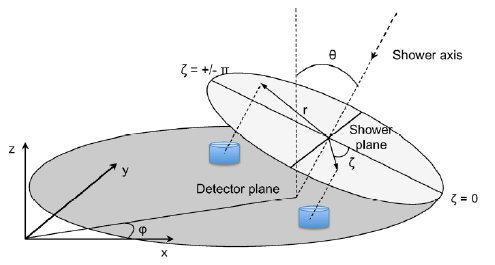
\includegraphics[width=0.7\textwidth]{capitulos/imagenes_capitulos/cap3/esquema_lluvia.png} 
	\caption{Esquema geométrico de una Lluvia Atmosférica Extensa (EAS). Se ilustra la proyección de las posiciones de los detectores desde el plano del suelo hacia el plano de la lluvia, definiendo las coordenadas intrínsecas $r$ y el ángulo azimutal $\phi$ (en el dibujo escrita como $\zeta$) del plano de la lluvia.}
	\label{fig:plano_lluvia}
\end{figure}

En el caso ideal de una lluvia estrictamente vertical ($\theta = 0^\circ$), ambos planos coinciden de manera exacta. En esta configuración, la distancia de vuelo que recorren las partículas desde el punto de primera interacción hasta alcanzar el nivel del suelo depende exclusivamente de la distancia radial al núcleo ($r$). Por lo tanto, los detectores ubicados a una misma distancia $r$ registrarán, en promedio, idénticas densidades de muones, reflejando una simetría circular independiente del ángulo azimutal ($\phi$).

Sin embargo, cuando el rayo cósmico primario incide con un ángulo cenital $\theta > 0^\circ$, el plano de la lluvia deja de ser paralelo al plano del suelo. Esta inclinación geométrica rompe inherentemente la simetría del sistema respecto al observador terrestre.

Para comprender esta ruptura geométrica, es necesario analizar la intersección del frente de la lluvia con la superficie del arreglo. Al inclinar la cascada, los detectores ubicados a una misma distancia radial $r$ en el plano de la lluvia ya no se encuentran a la misma distancia física del centro de la lluvia en el plano del suelo, ni tampoco del máximo de desarrollo de la lluvia ($X_{max}$). Por ende las distintas partículas que componen la lluvia no son recorren caminos idénticos antes de impactar contra el suelo. Esto define dos regiones azimutales extremas y fundamentales para el análisis de asimetrías:

\begin{itemize}
	\item \textbf{Región Temprana ($\phi \approx 0^\circ$):} Corresponde a la sección del frente de lluvia que se encuentra más cerca de la superficie topográfica (el suelo) y, por ende, impacta primero contra el arreglo de detectores. Las partículas que arriban a esta zona tienen el camino geométrico más corto y recorren la menor cantidad de atmósfera.
	\item \textbf{Región Tardía ($\phi \approx \pm 180^\circ$):} Corresponde a la sección diametralmente opuesta del frente, la cual se encuentra `elevada' respecto al suelo. Las partículas en esta dirección deben continuar propagándose a través de la atmósfera después de que el lado \textit{temprano} ya ha impactado, acumulando una distancia atravesada en la atmósfera significativamente mayor antes de ser detectadas y por ende siendo más atenuadas.
\end{itemize}

Esta diferencia estructural de origen geométrico en las distancias de propagación para un mismo radio $r$ justifica junto a otras razones, los fenómenos físicos responsables de modular la densidad de muones, los cuales se describen a continuación.

\subsection{Origen físico de la modulación azimutal}
\label{subsec:origen_fisico}

La ruptura de la simetría circular detallada anteriormente es el resultado de la superposición de tres mecanismos físicos y cinemáticos que actúan sobre la cascada durante su desarrollo y propagación.  Si bien la asimetría dominante en este trabajo es de tipo \textit{temprano-tardía}, es fundamental caracterizar cada una de las 3 contribuciones \cite{GAP2007_124} para comprender la firma total de la densidad de muones a nivel del suelo.

\subsubsection{Atenuación atmosférica}
\label{subsubsec:atenuacion}

La atenuación longitudinal es consecuencia de la evolución de la cascada a través del medio. Como se estableció en la Sección \ref{subsec:simetria_ruptura}, las partículas en la región tardía deben atravesar una profundidad atmosférica mayor que aquellas en la región temprana cuando la lluvia esta inclinada, es decir, no es estrictamente vertical. Esto se puede entender al considerar que la parte temprana de la lluvia impacta contra el suelo '\textit{antes}' que la tardía, y por ende esta ultima atraviesa más atmósfera. Este es el efecto dominante que afecta a la componente muónica de las lluvias detectadas en el UMD en el rango angular estudiado.

Dado que la cascada evoluciona y se absorbe a medida que penetra en la atmósfera, este camino extra resulta en un vaciamiento relativo de partículas en la zona tardía. Físicamente, la atenuación genera un exceso de densidad de muones en la dirección $\phi = 0^\circ$ temprana respecto de la zona tardía. Este fenómeno ha sido ampliamente documentado en simulaciones y datos experimentales del SD \cite{Pryke1998, BradfieldThesis}. Vale aclarar que este fenómeno ocurre tanto para la componente electromagnética como la muónica pero con mayor magnitud para la componente EM, razón por la cual este mecanismo ya estaba caracterizado.

Si bien los muones poseen un gran poder de penetración y menor sección eficaz de interacción que la componente de $e^{-}/\gamma$, el efecto tiene un impacto relevante para esta componente de la lluvia. A grandes distancias del núcleo ($r > 400 \text{ m}$), el espectro muónico está dominado por partículas de menor energía (muones blandos) \cite{Cazon2012}. En este régimen, la probabilidad de decaimiento aumenta sensiblemente con el trayecto adicional hacia la región tardía, consolidando la atenuación atmosférica como el efecto dominante para la componente muónica pura. En este contexto, el blindaje de tierra de 2.3 m del UMD cumple un rol fundamental: actúa como un filtro cinemático que elimina los muones sub-GeV que han sufrido atenuaciones extremas como también a la componente EM, permitiendo una medición más limpia de la asimetría intrínseca de los muones que logran penetrar el suelo.

\subsubsection{Efectos geométricos}
\label{subsubsec:divergencia}

El segundo fenómeno es de naturaleza puramente geométrica y cinemática. Surge de la relación entre la distribución angular intrínseca de las partículas y las distancias que deben recorrer para impactar en el plano del suelo.

Para comprender este efecto, primero es necesario analizar la cinemática de producción de muones. En la cascada hadrónica, los muones nacen a una cierta altura $z$ producto del decaimiento de piones y kaones. En este proceso, heredan un momento longitudinal $p_z$ y un momento transversal $p_t$. De acuerdo con el modelo cinemático descrito por L. Cazón \textit{et al.} \cite{Cazon2012}, este momento transversal provoca que el muón salga disparado con un ángulo de apertura polar $\alpha$ respecto al eje de la lluvia. La relación trigonométrica fundamental está dada por $\sin \alpha \simeq c p_t / E$. Bajo la aproximación de ángulos pequeños, la distancia radial $r$ a la que impactará el muón en el plano ortogonal (plano de la lluvia) depende de este ángulo de apertura:

\begin{equation}
	r = z \tan \alpha \approx z \sin \alpha \approx z \left( \frac{c p_t}{E} \right) \approx z \left( \frac{p_t}{p_z} \right)
\end{equation}

Al propagar el haz de partículas hacia el suelo, la densidad de muones $S$ que registrará un detector depende de dos factores cinemáticos que compiten entre sí. Por un lado, la densidad espacial cae con el cuadrado de la distancia geométrica recorrida ($1/d^2$), dado que el área transversal interceptada crece esféricamente como $dA = d^2 d\Omega$. Por otro lado, la cantidad de partículas emitidas en una dirección dada, $\frac{dN}{d\Omega}(\alpha)$, \textbf{decae abruptamente} a medida que se exigen ángulos $\alpha$ cada vez más extremos. Esto ocurre porque el espectro del momento transversal $p_t$ está fuertemente acotado por la cinemática de las interacciones hadrónicas (decayendo exponencialmente $\propto p_t \times \exp(-p_t/Q)$) \cite{Cazon2012}. De manera simplificada, la densidad en el suelo se expresa como:

\begin{equation}
	S(d, \alpha) \propto \frac{1}{d^2} \frac{dN}{d\Omega}(\alpha)
\end{equation}

En una lluvia inclinada, la geometría del sistema impone que para alcanzar una misma distancia radial $r$ en el plano de la lluvia, la región tardía se encuentra físicamente más lejos del punto de producción que la región temprana ($d_{tardio} > d_{temprano}$).

Esto obliga geométricamente a que el ángulo de emisión necesario para impactar en la zona tardía sea estrictamente menor ($\alpha_{tardio} < \alpha_{temprano}$). Dicho de manera más intuitiva, como la región temprana de la lluvia impacta contra el suelo primero, el muón recorre poca distancia (en la imagen $d_u$) y por ende requiere un ángulo $\alpha$ grande para alcanzar el radio $r$. Inversamente, como la región tardía impacta más lejos, le basta con un ángulo $\alpha$ significativamente más pequeño para alcanzar el mismo radio $r$. Este esquema se ilustra en la Figura \ref{fig:divergencia_angular}.

\begin{figure}[H]
	\centering
	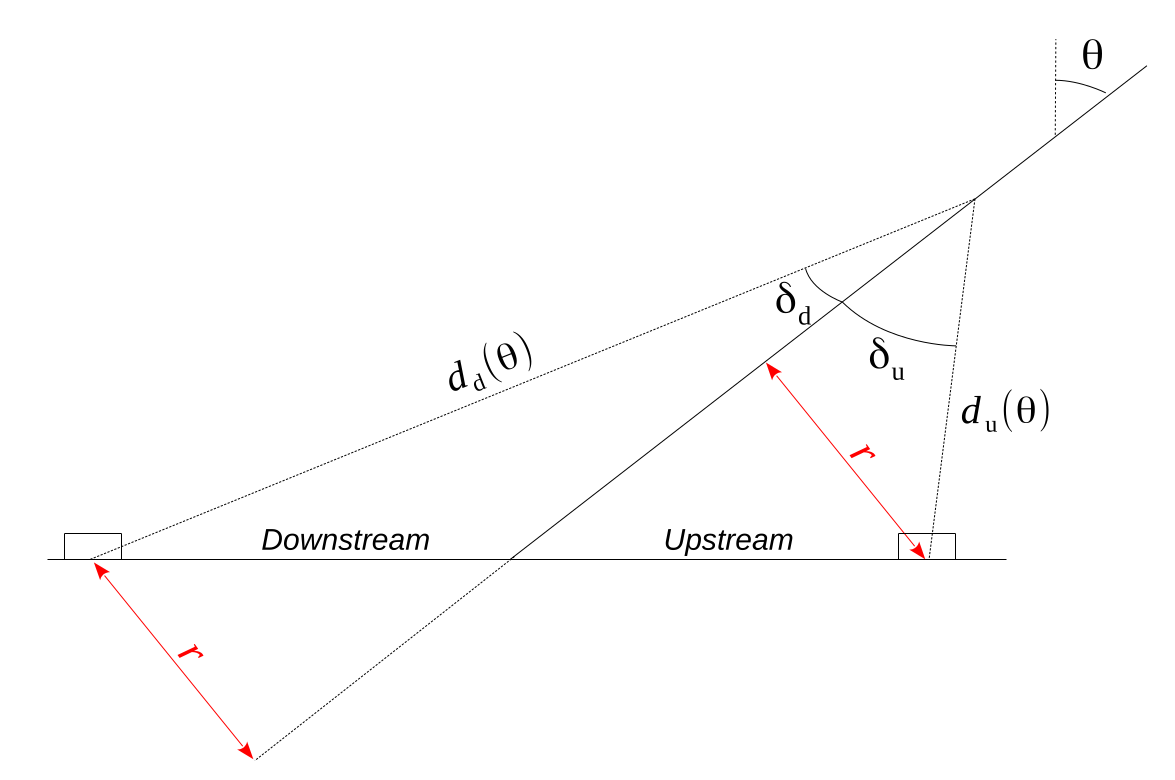
\includegraphics[width=1\textwidth]{capitulos/imagenes_capitulos/cap3/efecto_geo_luce_icrc2021.png} 
	\caption{Esquema geométrico de la dispersión de las partículas. Debido a la inclinación, para alcanzar un mismo radio $r$ en el plano de la lluvia, la región tardía requiere un ángulo de emisión $\alpha$ (en la imagen $\delta_d$) mucho menor que la región temprana (en la imagen $\delta_u$). Obtenido de \cite{Luce_ICRC2021}}
	\label{fig:divergencia_angular}
\end{figure}

Aquí es donde la distribución angular se vuelve determinante. Como la zona tardía requiere un ángulo $\alpha$ menor, queda alineada con una porción del haz intrínsecamente más densa. Dicho de otra manera, como $\alpha \approx p_t / p_z$, pedirle a un muón que tenga un ángulo $\alpha$ extremo implica exigirle un valor de $p_t$ estadísticamente  improbable. Esta masiva ganancia estadística de partículas al exigir un $\alpha$ menor compensa con creces la pérdida de densidad causada por la lejanía espacial (el factor $1/d^2$). En consecuencia, se proyecta un fuerte exceso artificial de densidad sobre la región tardía ($\phi = \pm 180^\circ$).

Como advirtió Billoir, un evento puramente simétrico en el sistema de referencia de la lluvia resulta en un efecto asimétrico al proyectarse en el plano del suelo. Para cuantificar esta excentricidad remanente, Bertou y Billoir desarrollaron una derivación analítica evaluando los momentos de las partículas \cite{GAP2000_017}. La modulación espuria aparente introducida por el mapeo espacial fue cuantificada mediante el término asimétrico $\mathcal{A}_{geo}$ que es lo que llamamos efecto geométrico:

\begin{equation}
	\mathcal{A}_{geo}(r, \Phi) = \left\langle \frac{p_r(r)}{-p_z(r)} \right\rangle \tan \theta \cos \Phi
	\label{eq:efecto_geo}
\end{equation}

donde $p_r$ es la componente radial del momento y $p_z$ la longitudinal. La implicancia de esta ecuación es crítica, la asimetría geométrica escala directamente con la tangente del ángulo de divergencia porque $\langle p_r / -p_z \rangle \approx \tan \alpha$. Además el valor de esta asimetría que tiene el mismo comportamiento funcional azimutal que la atenuación atmosférica, posee signo opuesto necesariamente.

Es precisamente en la evaluación de este término donde se hace necesario distinguir la composición espectral de la cascada, la cual exhibe una dicotomía fenomenológica en la componente muónica al considerar un radio fijo:

\begin{itemize}
	\item \textbf{Población A (Alta Energía):} Muones producidos a gran altura con un momento longitudinal inmenso ($p_z \gg p_t$). Su ángulo de divergencia $\alpha$ es minúsculo, resultando en un cociente $\langle p_r / -p_z \rangle$ muy cercano a cero.
	\item \textbf{Población B (Baja Energía):} Muones producidos más cerca del suelo con un momento longitudinal bajo ($p_z \sim p_t$). Su divergencia $\alpha$ es masiva, lo que provoca que el término asimétrico de Billoir explote a grandes distancias con signo negativo.
\end{itemize}

Es imperativo notar que el espectro de energía inicial $E_i$ de los muones decae fuertemente siguiendo una ley de potencias $E_i^{-2.6}$ \cite{Cazon2012}. Esto significa que la cascada está abrumadoramente dominada en número por la Población B de baja energía. Al estar la lluvia inundada por esta población altamente divergente, el factor geométrico escala de manera drástica con el radio y domina por completo la señal en detectores de superficie que no posean un umbral de energía.

Este fenómeno compite de manera directa contra el vaciamiento producido por la atenuación atmosférica, forzando la asimetría total observada hacia valores fuertemente negativos. A diferencia de la componente electromagnética (que se ensancha y difumina por dispersión múltiple de Coulomb a medida que interactúa con la atmósfera), los muones viajan en trayectorias casi rectilíneas por ser casi 200 veces más masivos.

La existencia de este fuerte artefacto topológico plantea un desafío, pero también revela una oportunidad experimental vinculada a los umbrales de detección. Si un instrumento es capaz de imponer un corte de energía estricto, actuaría como un filtro cinemático. Al eliminar por completo a la abundante Población B, aislaría exclusivamente las trayectorias colimadas de la Población A. Bajo esta restricción analítica donde $p_z \gg p_r$, el efecto geométrico de proyección colapsa matemáticamente a cero ($\lim_{p_z \to \infty} \mathcal{A}_{geo} \to 0$). Esta anulación analítica del efecto geométrico es el principio fundamental que subyace al desempeño del Detector Subterráneo de Muones y que será abordado en los resultados de esta tesis.

\subsubsection{Efectos por el campo geomagnético terrestre}
\label{subsubsec:geomagnetico}

Finalmente, la simetría se ve alterada por la acción de la fuerza de Lorentz sobre la componente cargada de la lluvia. El campo geomagnético terrestre ($\vec{B}$) induce una deflexión en la trayectoria de los muones según la relación $\vec{F} = q(\vec{v} \times \vec{B})$, separando lateralmente a los muones de cargas opuestas ($\mu^+$ y $\mu^-$).

Esta deflexión introduce una distorsión sistemática que se superpone a la asimetría temprano-tardía. Dado que el Observatorio Pierre Auger recibe lluvias con una distribución uniforme en el ángulo azimutal de incidencia ($\phi_{shower}$), el vector de la fuerza de Lorentz varía su orientación relativa respecto al plano de la lluvia en cada evento. Sin un filtrado o corrección por dirección de arribo, este fenómeno actúa como una fuente de ruido coherente que dispersa los valores de densidad medidos. En el marco de un ajuste armónico global, esta dispersión se manifiesta como una reducción espuria en la amplitud del parámetro $A_1$, subestimando la asimetría real inducida por la atenuación y la geometría. Para el rango de energías y ángulos cenitales aquí abordados, este efecto se considera de segundo orden.

Sin embargo, en el régimen de lluvias extremadamente inclinadas ($\theta > 80^\circ$), el largo camino atmosférico permite separaciones espaciales masivas entre muones positivos y negativos, convirtiendo a la deflexión magnética en el mecanismo dominante de asimetría. Estudios recientes presentados en la Reunión de la Colaboración Pierre Auger por M. Scornavacche \cite{Scornavacche2026} y otros \cite{collaboration_2014}, demuestran que esta deformación de los mapas muónicos es una herramienta potente para la discriminación de masa primaria en eventos horizontales, lo que resalta la importancia de caracterizar correctamente todas las fuentes de asimetría para complementar el análisis en lluvias de inclinación intermedia presentado en este trabajo.

\subsection{Parametrización armónica de primer orden}
\label{subsec:parametrizacion}

Para cuantificar esta ruptura de simetría en la Función de Distribución Lateral (LDF), Billoir et al. \cite{Billoir2002} propusieron la inclusión de una parametrización de modulación cosinusoidal. Siguiendo este formalismo, la densidad de partículas (o la señal del detector) en el plano de la lluvia se modela como una función armónica de primer orden:

\begin{equation}
	S(r,\phi) = \langle S(r) \rangle \left( 1 + A_1(r, \theta) \cos\phi \right)
	\label{eq:asimetria_a1}
\end{equation}

donde $\langle S(r) \rangle$ es la densidad promedio a la distancia $r$ para una lluvia completamente simétrica, $A_1$ representa la amplitud de la asimetría temprano-tardía, y $\phi$ es el ángulo azimutal de las estaciones en el plano de la lluvia. Un valor de $A_1 > 0$ indica dominancia de la atenuación atmosférica (pico en la región temprano), mientras que un $A_1 < 0$ señala la dominancia de efectos geométricos (pico en la región tardía).

Un objetivo central de este trabajo es también caracterizar la sensibilidad del parámetro $A_1$ respecto a la naturaleza del primario y la energía de la lluvia. Esta exploración es fundamental, ya que la amplitud de la asimetría está intrínsecamente vinculada al estado de desarrollo de la cascada y, por ende, constituye un estimador independiente de la composición de masa. Es importante destacar que esta parametrización asume que el mecanismo dominante en el rango de detección del UMD es la atenuación atmosférica, lo que se traduce en valores de $A_1$ positivos. Bajo esta premisa, y en concordancia con la metodología empleada para los detectores de superficie WCD y SSD \cite{BradfieldThesis}, se optó por fijar la fase de la modulación en $\phi_0 = 0$. Esta restricción impone que el eje de simetría de la asimetría coincida con la línea temprano-tardía, maximizando la sensibilidad del ajuste al desarrollo longitudinal de la lluvia.

Históricamente, el estudio de asimetrías azimutales en el Observatorio Pierre Auger se ha centrado en las señales medidas por el Detector de Superficie (SD) por ser el detector inicial del Observatorio. Los primeros estudios fenomenológicos como los de Pryke \cite{Pryke1998} y Billoir et al. \cite{Billoir2002} identificaron los patrones de asimetría en estaciones Cherenkov. Recientemente, con la actualización AugerPrime, Bradfield \cite{BradfieldThesis} realizó análisis sistemáticos utilizando los detectores de superficie centelladores (SSD) combinados con los WCD, corroborando la utilidad de estas asimetrías para estudios de composición de masa.

Sin embargo, debido a que la señal del SD está invariablemente dominada por la componente electromagnética a los ángulos cenitales considerados, la magnitud intrínseca y la fenomenología de la asimetría temprano-tardía para una señal pura de muones duros ha permanecido inexplorada y no necesariamente esperamos que se comporte de manera estrictamente análoga. Abordar este vacío utilizando las capacidades del UMD como detector específicamente de muones, es el propósito central de los siguientes capítulos.

\newpage


\clearpage
\setcounter{section}{4}
\phantomsection\label{review:05}
% !TEX root = ../main.tex

\section{Caracterización de la Asimetría en el Anillo Denso}
\label{sec:cap_anillo_denso}

En este capítulo se presentan los resultados obtenidos a partir del análisis de la asimetría azimutal en la densidad de muones utilizando la configuración de \textit{Anillo Denso}. Este marco permite estudiar la respuesta del detector y la física de la cascada en condiciones controladas, minimizando las incertidumbres vinculadas a la caída radial de la densidad de partículas. Además, este estudio permite mitigar las fluctuaciones estadísticas que podrían presentarse debido a la distribución física irregular de las estaciones en el terreno, garantizando una alta estadística por bin azimutal. Se analizan la estabilidad del parámetro $A_1$, los efectos sistemáticos de la reconstrucción y, finalmente, la capacidad de este observable para la discriminación de la masa del rayo cósmico primario.

\subsection{El Anillo Denso como entorno de control}
\label{subsec:entorno_control}

La configuración de Anillo Denso representa el escenario ideal para caracterizar la modulación azimutal. Al situar 12 estaciones virtuales a una distancia radial fija de $r = 450$~m en el plano de la lluvia, se garantiza que cualquier variación en la señal detectada sea independiente de la Función de Distribución Lateral (LDF). 

En este contexto, la densidad de partículas $S$ se modela mediante un ajuste armónico de primer orden:

\begin{equation}
	S(\phi) = \langle S \rangle (1 + A_1 \cos\phi)
	\label{eq:ajuste_armonico}
\end{equation}

donde $\phi$ es el ángulo azimutal de la estación en el plano de la lluvia, $\langle S \rangle$ es la densidad media en el anillo y $A_1$ es la amplitud de la asimetría. Como se discutió en el Capítulo 3, un valor de $A_1 > 0$ indica una dominancia del efecto de atenuación atmosférica (exceso en la zona temprana, $\phi = 0^\circ$), mientras que un $A_1 < 0$ reflejaría la dominancia de efectos geométricos y de divergencia radial (exceso en la zona tardía, $\phi = \pm 180^\circ$). 

Dado que a $r = 450$~m el sistema se encuentra fuera de la región de dominancia geométrica pura ($r < 200$~m), se espera que la contribución de los efectos de atenuación atmosférica prevalezca frente a los efectos de divergencia, permitiendo una medición estable y positiva de $A_1$.

En la Figura \ref{fig:ejemplo_ajuste} se presenta un ejemplo del ajuste realizado para una muestra de protones (modelo hadrónico \texttt{Sibyll 2.3e}) en el bin de mayor inclinación ($59.3^\circ < \theta_{\text{shower}} < 65^\circ$). Los datos corresponden a la cantidad de muones reconstruida por el UMD ($N^{\text{REC}}_\mu$). Se observan las doce estaciones virtuales equiespaciadas, donde las barras de error representan la desviación estándar estadística de la media. Se aprecia una modulación clara donde la diferencia de señal entre el máximo (región temprana) y el mínimo (región tardía) es de aproximadamente un 14\% ($\pm 7\%$ respecto a la media), confirmando una ruptura de simetría significativa para la componente muónica.

Este análisis se extendió usando también los datos de tanto la cantidad de muones inyectados por CORSIKA ($N^{\text{MC}}_\mu$) como la señal total registrada por los detectores de superficie (SD), permitiendo una comparación directa con estudios previos \cite{BradfieldThesis}. Para todos los datos se usaron las posiciones de las estaciones obtenidas a partir de la reconstrucción.

\begin{figure}[H]
	\centering
	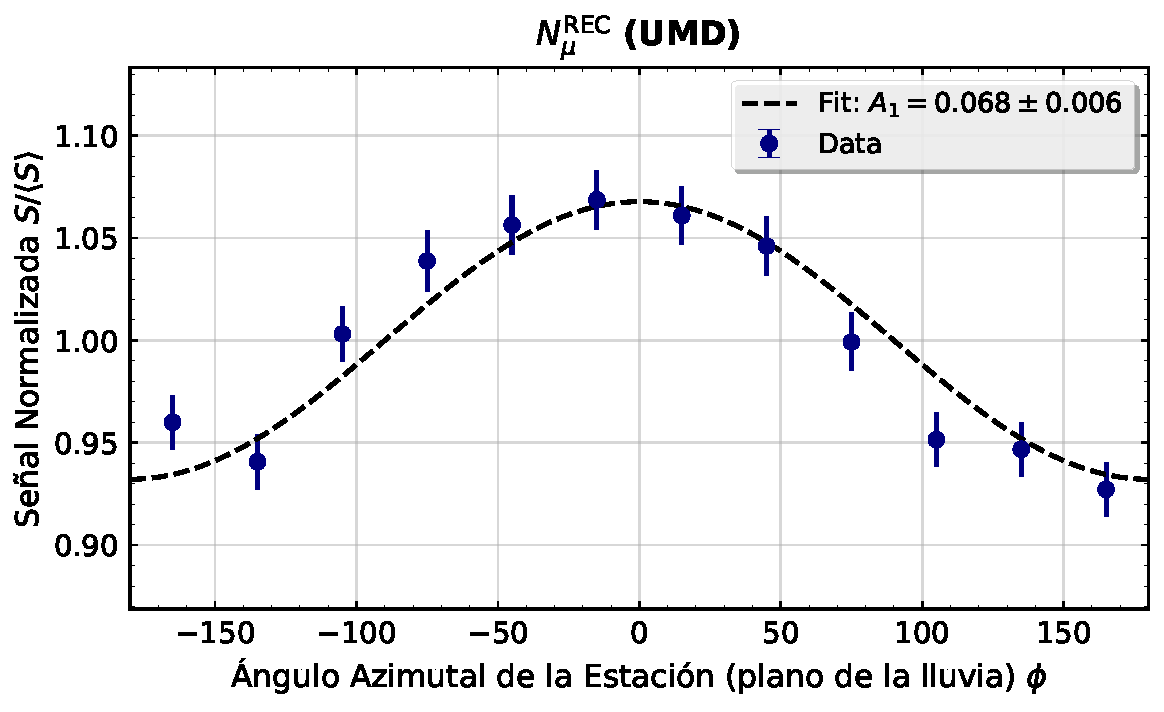
\includegraphics[width=1\textwidth]{capitulos/imagenes_capitulos/cap5/Ajuste_UMD_REC_Bin9.pdf}
	\caption{Ejemplo del ajuste armónico aplicado a la densidad de muones en el Anillo Denso para eventos de protón (\texttt{Sibyll 2.3e}). Los puntos representan las 12 estaciones virtuales y la curva sólida el ajuste del parámetro $A_1$ según la Ec. \ref{eq:ajuste_armonico}.}
	\label{fig:ejemplo_ajuste}
\end{figure}

 Es importante distinguir la naturaleza de los observables: mientras que el UMD cuantifica puramente la cantidad de muones, el SD registra la energía depositada total en unidades VEM (\textit{Vertical Equivalent Muon}) \cite{auger2015detector}. Esta es una unidad de energía normalizada propia del detector que considera la energía depositada de todas las partículas que atraviesan el SD, ya sean pertenecientes a la componente muónica como electromagnética de la lluvia. La evolución de $A_1$ para todos los bines cenitales se resume en la Figura \ref{fig:evolucion_asym_vs_theta}.

Al comparar las curvas, se observa que el SD presenta valores de asimetría significativamente mayores en bines de baja inclinación cenital, pero sufre un decaimiento abrupto a partir de $\theta_{\text{shower}} \gtrsim 50^\circ$. 

Este comportamiento es consistente con la fenomenología de la cascada: en lluvias más verticales, la señal del SD está dominada por la componente electromagnética (electrones y fotones), que es órdenes de magnitud más numerosa que la muónica. La discrepancia en la magnitud de la asimetría entre el SD y el UMD se fundamenta en la naturaleza de los procesos de pérdida de energía de estas partículas secundarias. La componente electromagnética está gobernada por procesos de \textit{bremsstrahlung} y creación de pares. Estos procesos están caracterizados por una longitud de radiación muy corta en la atmósfera, lo que provoca una atenuación exponencial rápida tras superar el máximo de la cascada. En contraste, los muones poseen una sección eficaz para la radiación de frenado mucho menor, dado que esta es inversamente proporcional al cuadrado de la masa. En consecuencia, pierden energía principalmente mediante ionización continua a una tasa mucho más baja y estable \cite{gaisser2016}. Esta diferencia en el poder de penetración explica por qué la amplitud $A_1$ es significativamente mayor en el SD (dominado por la atenuación abrupta de la componente EM) que en el UMD (que detecta puramente la componente muónica altamente penetrante).

\begin{figure}[H]
	\centering
	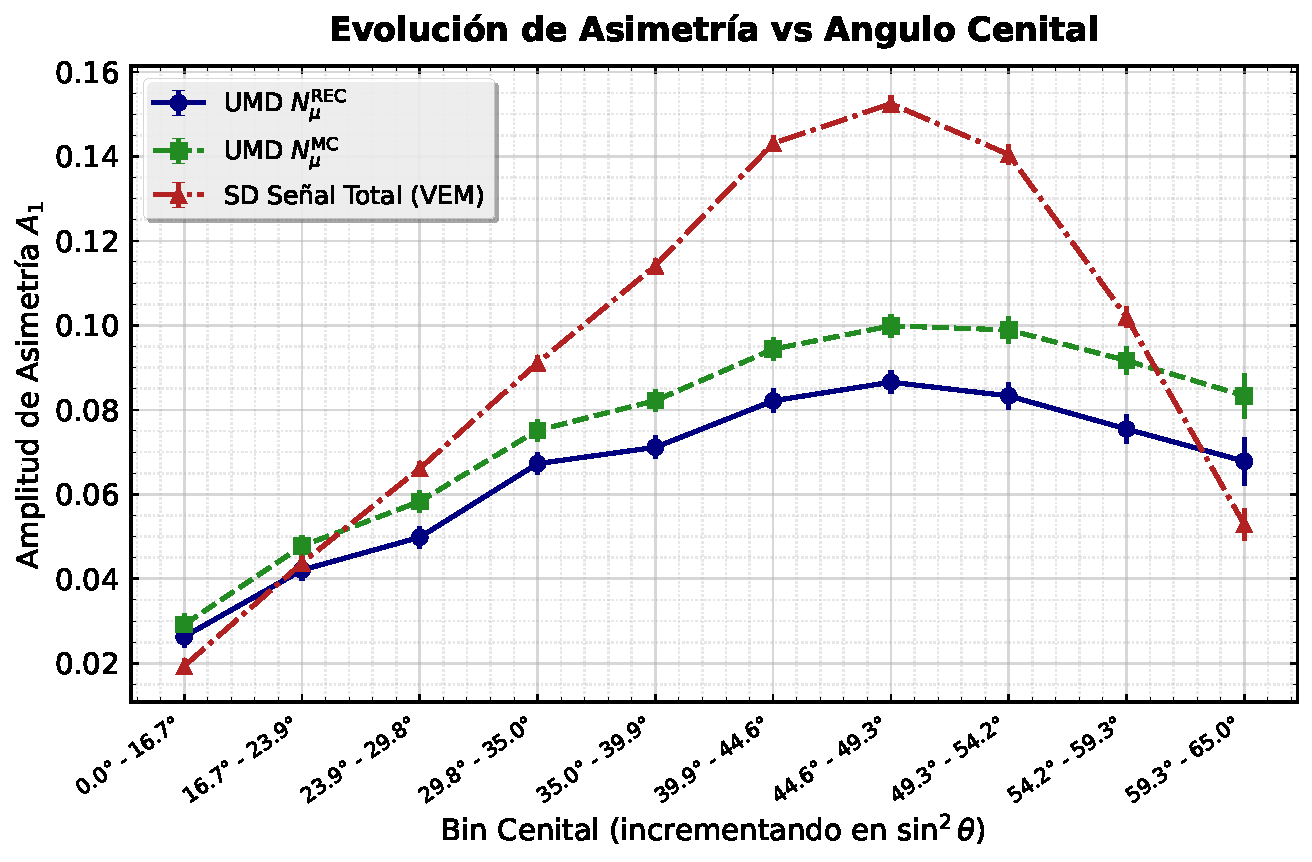
\includegraphics[width=1\textwidth]{capitulos/imagenes_capitulos/cap5/Evolucion_Asimetria_vs_Theta.pdf}
	\caption{Evolución de la amplitud $A_1$ con su error en función de $\theta$ para el UMD (REC en azul, MC en verde) y el SD (rojo). Se observa la inversión de dominancia entre el SD y el UMD a altas inclinaciones.}
	\label{fig:evolucion_asym_vs_theta}
\end{figure}

Sin embargo, a medida que aumenta la inclinación, el espesor atmosférico recorrido crece de forma no lineal, provocando que la componente EM sea casi totalmente absorbida antes de alcanzar el nivel del suelo. En este régimen de alta inclinación, la señal del SD pasa a estar dominada exclusivamente por muones, lo que explica la caída de la asimetría medida a niveles comparables o inferiores a los del UMD. El hecho de que el $A_1$ del SD caiga incluso por debajo de los valores del UMD se atribuye a la presencia de muones de baja energía. Tal como se demuestra en el modelo de transporte cinemático \cite{Cazon2012}, estos muones de baja energía dominan a grandes distancias del núcleo y a mayores ángulos cenitales, sufriendo mayores deflexiones y retrasos geométricos. Como consecuencia, estas partículas de baja energía tienden a poblar de manera asimétrica la región tardía, lavando la asimetría de atenuación atmosférica positiva que sí logran preservar los muones más energéticos filtrados por el blindaje del UMD.

Finalmente, se observa una discrepancia sistemática entre los valores de asimetría $A_1$ obtenidos para los muones reconstruidos ($N^{\text{REC}}_\mu$) y los muones inyectados ($N^{\text{MC}}_\mu$) en el UMD. Esta diferencia, que indica un lavado o subestimación de la asimetría introducido por el framework de reconstrucción \textit{Offline}, será analizada en detalle en la sección \ref{subsec:mc_vs_rec}.

\subsection{Efectos Sistemáticos: Discrepancias MC vs. REC}
\label{subsec:mc_vs_rec}

Como se evidenció en la Figura \ref{fig:evolucion_asym_vs_theta}, existe una diferencia sistemática persistente entre la amplitud de asimetría $A_1$ obtenida a partir de muones inyectados ($N^{\text{MC}}_\mu$) y muones reconstruidos ($N^{\text{REC}}_\mu$). Dado que este análisis se realiza utilizando la geometría controlada del Anillo Denso, se descartan errores de paralaje o de reconstrucción del núcleo como fuente de la discrepancia. Por lo tanto, el origen del sesgo debe buscarse en la respuesta del algoritmo de reconstrucción del UMD o en la validez de los ajustes.

En primera instancia, se evaluó la convergencia y estabilidad de los ajustes armónicos mediante la métrica de bondad de ajuste $\chi^2_\nu$. Los resultados para todos los bines cenitales se presentan en la Figura \ref{fig:chi_cuadrado_reducido}.

Para los datos del UMD, tanto en el nivel de simulación como de reconstrucción, se obtuvieron valores de $\chi^2_\nu \approx 1$. Esto confirma que el modelo armónico de primer orden describe adecuadamente la modulación muónica y que los ajustes son estadísticamente robustos. Esto permite descartar una inestabilidad del ajuste como la fuente de la diferencia ente los valores de asimetría del UMD.

\begin{figure}[H]
	\centering
	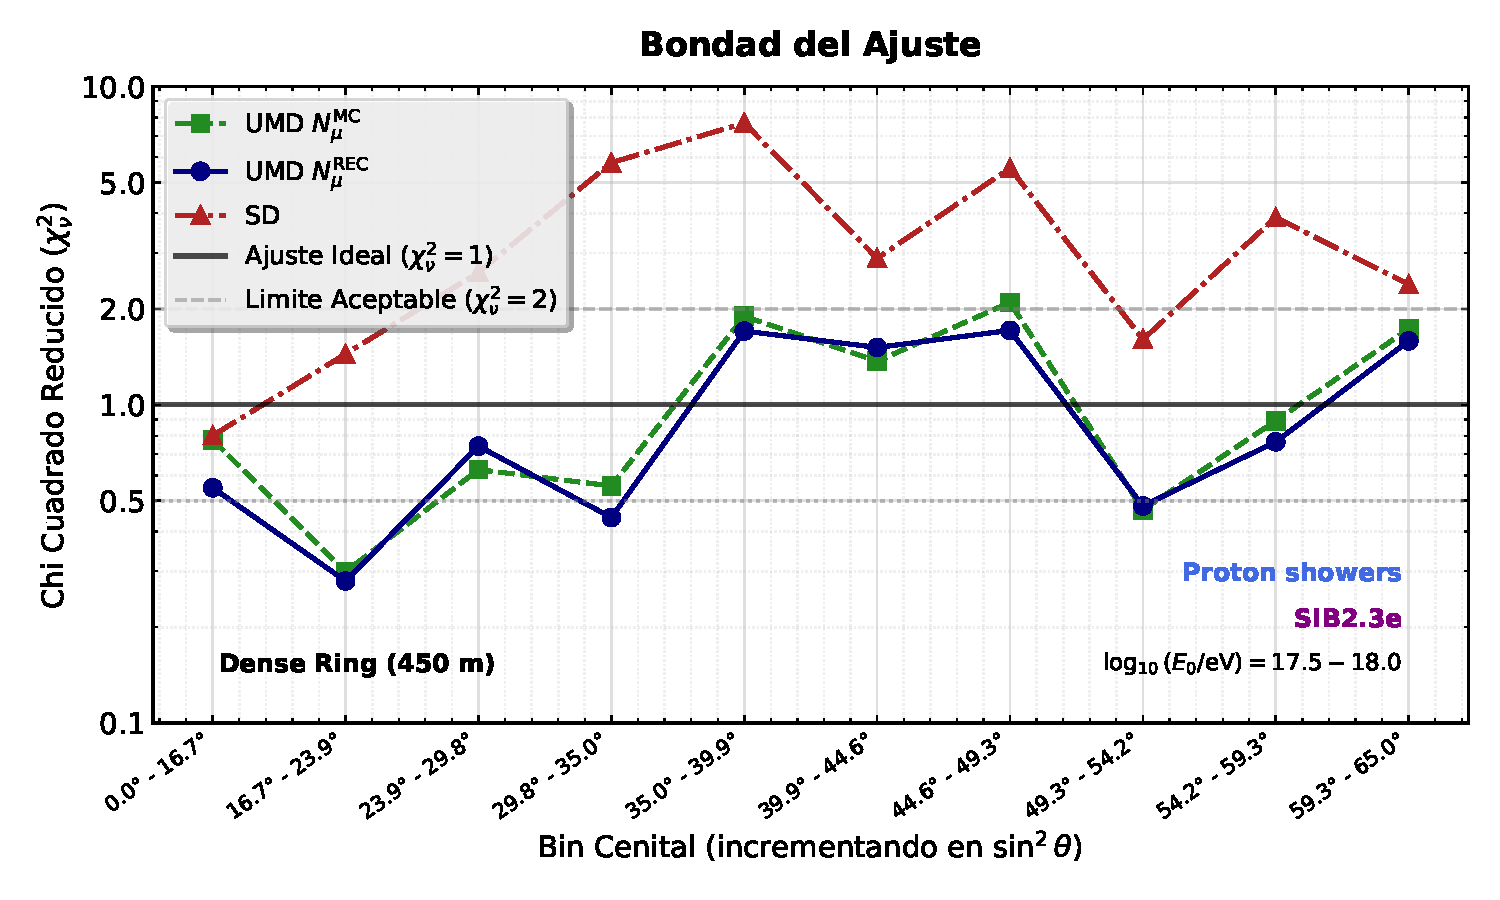
\includegraphics[width=1\textwidth]{capitulos/imagenes_capitulos/cap5/Chi2_Reduced_Fits.pdf}
	\caption{Bondad de ajuste $\chi^2_\nu$ para los bines cenitales. Se observa que los ajustes del UMD (REC y MC) se mantienen cercanos a la unidad, mientras que el SD presenta valores elevados debido a la alta precisión estadística de la muestra.}
	\label{fig:chi_cuadrado_reducido}
\end{figure}

Por el contrario, los ajustes del SD presentan valores de $\chi^2/\text{ndf}$ significativamente mayores (alcanzando un máximo de $\sim 10$). Este comportamiento no implica un fallo del modelo, sino que es consecuencia de la elevada estadística de la muestra (dado que la cantidad de partículas que llegan a los detectores es mucho mayor). Al ser el error de la media extremadamente pequeño, el test de $\chi^2$ se vuelve sensible a desviaciones de segundo orden o pequeñas asimetrías físicas que el modelo armónico simple no pretende capturar. La inspección visual del ajuste en el SD (ver Figura \ref{fig:anexo_ajuste_sd_bin9} en el Anexo \ref{anexo:ajustes_anillo_denso}) confirma que la curva describe la tendencia general de los datos con precisión, pero la rigurosidad estadística del $\chi^2$ penaliza los residuos mínimos que resultan significativos ante tan baja incertidumbre.

Para investigar la discrepancia en $A_1$ dentro del UMD, se analizó el rendimiento del algoritmo de reconstrucción de muones a nivel de estación. Se definió el Residuo Relativo de Muones como:

\begin{equation}
	\text{Residuo Relativo} = \frac{N^{\text{REC}}_\mu - N^{\text{MC}}_\mu}{N^{\text{MC}}_\mu}
\end{equation}

Esta métrica permite cuantificar el sesgo en el conteo de partículas de manera normalizada. La distribución de este residuo para la muestra de protones (\texttt{Sibyll 2.3e}) se muestra en la Figura \ref{fig:bias_umd_global}.

Si bien la distribución está centrada cerca del cero con una resolución aceptable, presenta una asimetría marcada respecto del cero. Mientras que el error por sub-reconstrucción está limitado físicamente (el residuo no puede ser menor a -1), el algoritmo presenta una cola de sobre-reconstrucción donde el número de muones detectados puede superar ampliamente al inyectado. Este fenómeno de 'sobreconteo' es intrínseco a los algoritmos de reconstrucción.

\begin{figure}[H]
	\centering
	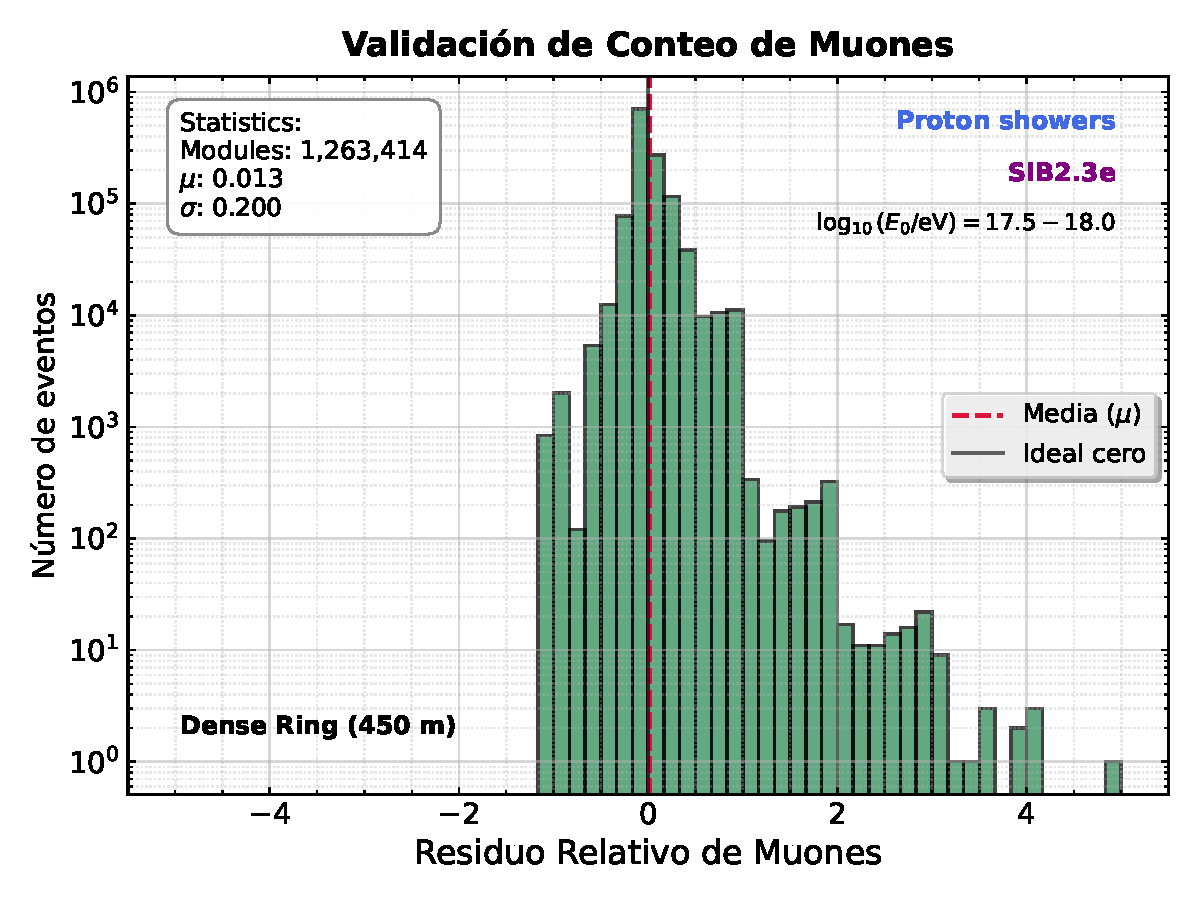
\includegraphics[width=1\textwidth]{capitulos/imagenes_capitulos/cap5/muon_counting_validation.pdf}
	\caption{Distribución del residuo relativo en la reconstrucción de muones. Aunque la media es cercana a cero, se observa una asimetría intrínseca con una cola extendida hacia la sobre-reconstrucción de partículas.}
	\label{fig:bias_umd_global}
\end{figure}

Se intento ver si esta asimetría de la distribución respecto del cero podía explicar las diferencias de la amplitud de asimetría $A_1$ entre los datos REC y los datos MC. Para esto se construyo un modelo que implementase la distribución encontrada en la Figura \ref{fig:bias_umd_global} en los datos. Sin embargo, este procedimiento solo inyectó ruido estadístico en los ajustes, sin lograr desplazar los valores de $A_1^{\text{MC}}$ hacia los niveles de $A_1^{\text{REC}}$. Este resultado negativo sugiere que el sesgo de reconstrucción no es uniforme, sino que posee una dependencia funcional con, por ejemplo, la posición de la estación o la densidad local de partículas.

\subsubsection{Bias Direccional en la Reconstrucción}
\label{subsec:bias_direccional}

Se planteó la hipótesis de que el error de conteo del UMD no es uniforme, sino que presenta una dependencia con la región azimutal de la lluvia. Si el sobreconteo es proporcionalmente mayor en las zonas de baja densidad ($\phi \approx \pm 180^\circ$) que en las de alta densidad ($\phi \approx 0^\circ$), el efecto resultante sería un aumento artificial del 'piso' de la señal tardía. Esto reduciría la modulación relativa entre ambas regiones, resultando en una degradación sistemática de la amplitud $A_1$ reconstruida.

Para verificar esta premisa, se estudió la evolución del valor medio del residuo relativo para lluvias inclinadas ($40^\circ \le \theta_{\text{shower}} \le 65^\circ$) particionando la muestra en 12 bines azimutales equiespaciados en el plano de la lluvia. Los resultados se presentan en la Figura \ref{fig:bias_direccional_rec}.

\begin{figure}[H]
	\centering
	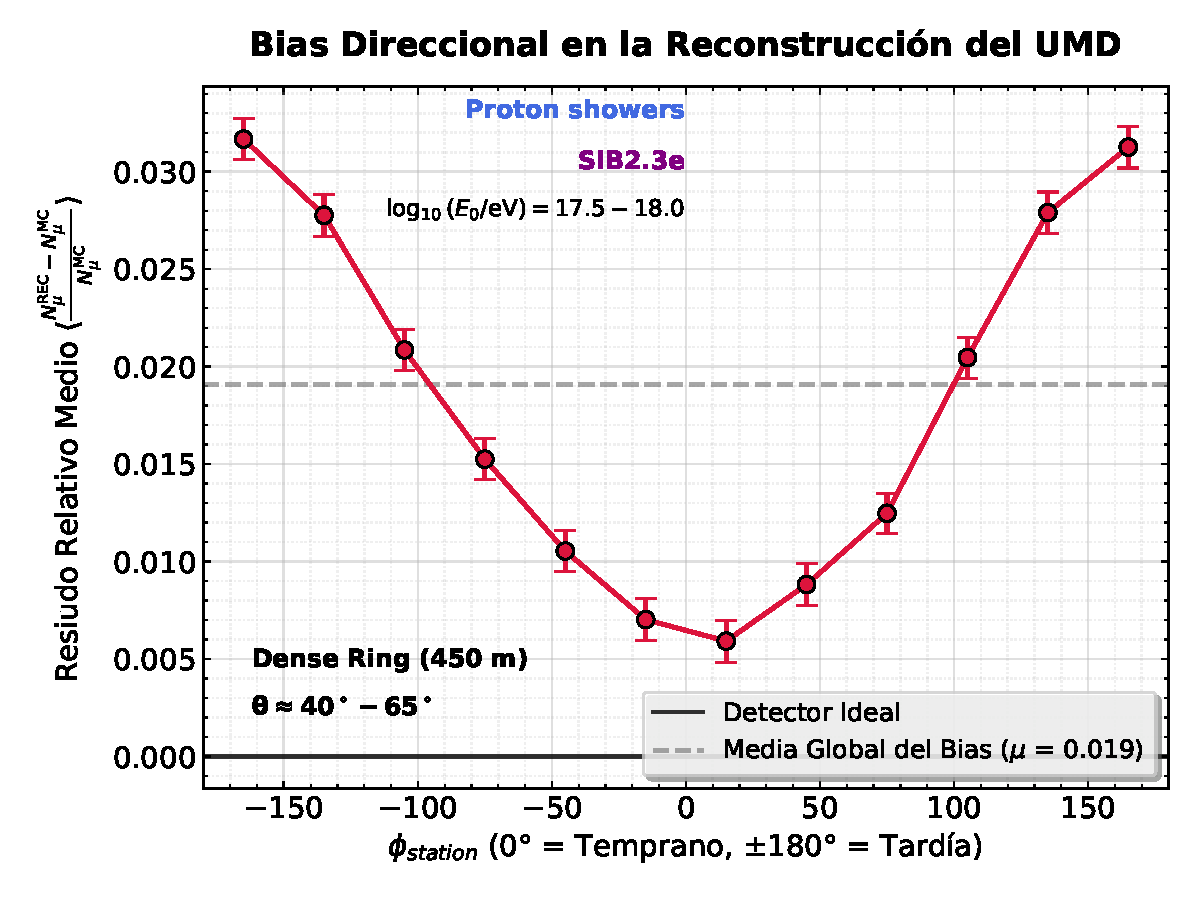
\includegraphics[width=1\textwidth]{capitulos/imagenes_capitulos/cap5/directional_bias.pdf}
	\caption{Distribución de la media del residuo relativo de reconstrucción en función del ángulo azimutal de la estación en el plano de la lluvia. Se evidencia un desempeño degradado en las regiones tardías ($\pm 180^\circ$), donde el sesgo de sobreconteo es máximamente superior al de la región temprana ($0^\circ$).}
	\label{fig:bias_direccional_rec}
\end{figure}
	
Como se observa, el algoritmo de reconstrucción presenta un sesgo positivo significativamente mayor en las regiones tardías. Físicamente, esto se debe a que en las zonas de menor densidad, cualquier fluctuación estadística o error en la deconvolución de trazas tiene un impacto relativo mucho mayor sobre el valor medio, elevando artificialmente la densidad de muones allí donde la atenuación atmosférica debería ser máxima. Este efecto actúa como un ruido coherente que 'lava' la asimetría física intrínseca de la cascada.

\subsubsection{Modelado del Bias: Implementación del \textit{Toy Model} empírico}
\label{subsec:toy_model}

Para caracterizar el impacto del error de reconstrucción en la amplitud medida y verificar si el sesgo direccional es suficiente para explicar la discrepancia observada entre los datos ideales y los reconstruidos, se implementó un \textit{Toy Model} de perturbación. Este modelo utiliza un enfoque de remuestreo empírico computacional, conocido como \textit{Bootstrap} \cite{efron1979bootstrap}. 

El algoritmo toma las densidades muónicas ideales ($N_{\mu}^{\text{MC}}$) en cada bin azimutal y les inyecta un factor de error extraído aleatoriamente de la distribución real de residuos relativos evaluada en la Figura \ref{fig:bias_direccional_rec} segmentados por $\phi$. Esta metodología garantiza dos condiciones físicas fundamentales: respeta estrictamente el límite de sub-reconstrucción (dado que el detector no puede reconstruir cantidades negativas de muones, el residuo empírico extraído siempre está acotado en un mínimo de $-1$), y captura con total fidelidad la cola asimétrica de sobreconteo característica del algoritmo del UMD. 

De esta manera, se evalúa la degradación resultante en $A_1$ considerando exclusivamente el efecto del ruido de conteo direccional, aislándola de otras fuentes de incertidumbre como la reconstrucción del núcleo, permitiendo su comparación directa con la asimetría reconstruida ($A_1^{\mathrm{REC}}$). Los resultados de este modelo se observan en la Figura \ref{fig:toy_model}.

\begin{figure}[H]
	\centering
	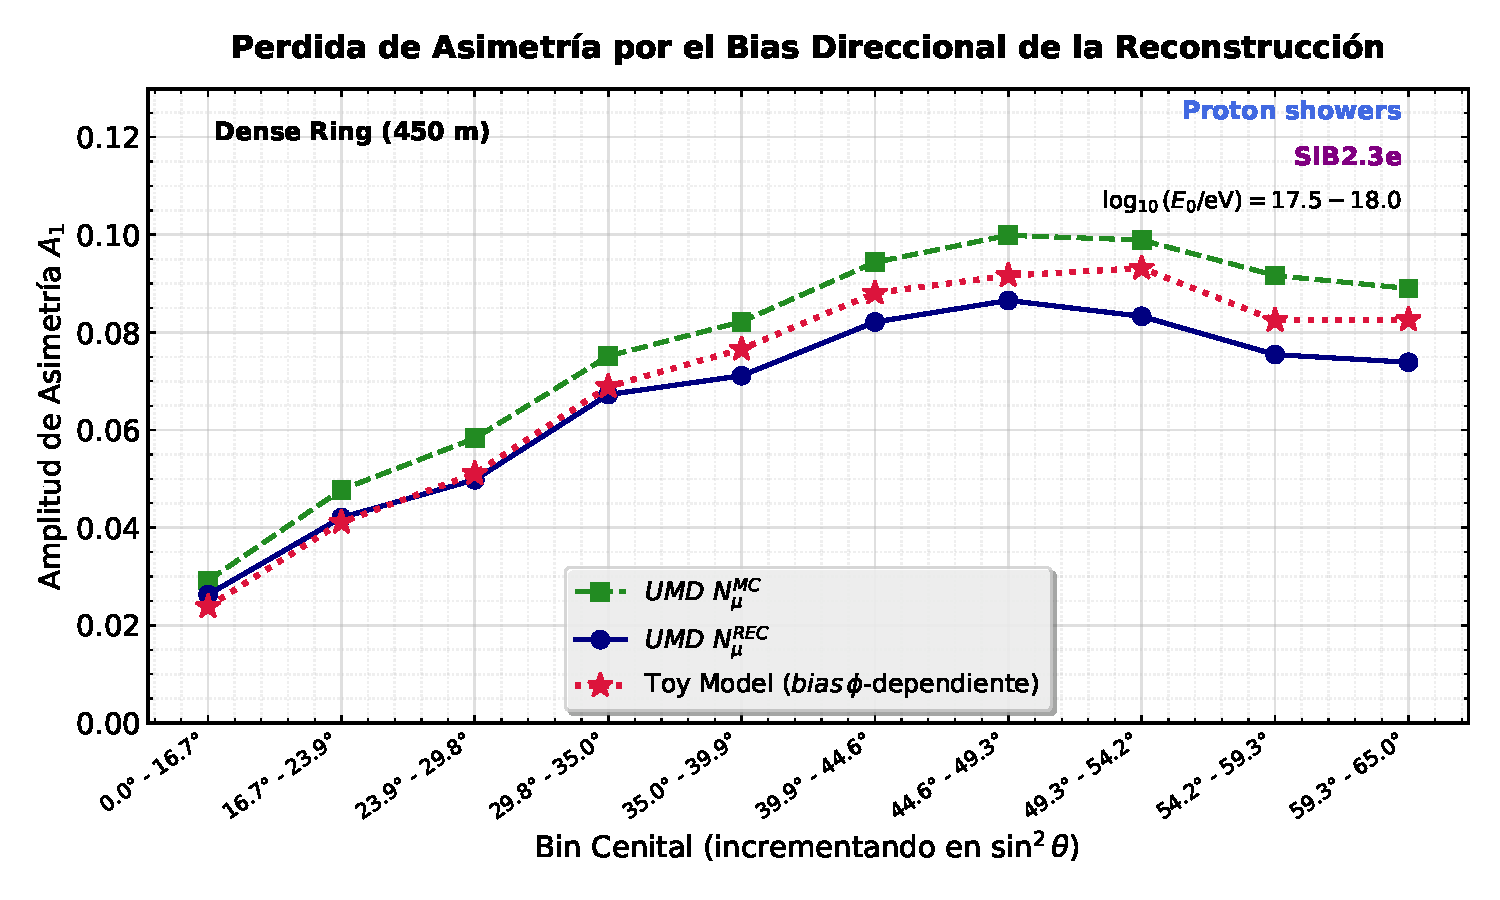
\includegraphics[width=1\textwidth]{capitulos/imagenes_capitulos/cap5/toy_model.pdf}
	\caption{Comparación de la amplitud de asimetría $A_1$ para muones inyectados (verde), reconstruidos (azul) y el resultado del \textit{Toy Model} direccional (rojo). Se aprecian dos regímenes diferenciados de degradación de señal según la inclinación de la cascada.}
	\label{fig:toy_model}
\end{figure}

El análisis de estos resultados demuestra que el \textit{Toy Model} logra reproducir el comportamiento de los datos reconstruidos, diferenciándose en dos grandes regímenes cinemáticos:

\begin{itemize}
	\item \textbf{Régimen cuasi-vertical ($\theta \lesssim 35^\circ$):} La amplitud de asimetría generada por el \textit{Toy Model} direccional se superpone casi con exactitud sobre la curva de la reconstrucción del detector ($A_1^{\mathrm{REC}}$). Esto constituye una evidencia robusta de que, en bines de baja inclinación, la totalidad de la pérdida de asimetría se origina en el sesgo de sobreconteo direccional del algoritmo de reconstrucción.
	\item \textbf{Régimen de media y alta inclinación ($\theta \gtrsim 35^\circ$):} Si bien el sesgo direccional introducido logra explicar más del 50\% de la degradación observada frente a los datos ideales, la curva del \textit{Toy Model} no alcanza a replicar la totalidad de la caída en $A_1^{\mathrm{REC}}$. Esta divergencia remanente en el régimen más inclinado indica la presencia de efectos topológicos o cinemáticos de segundo orden, tales como el \textit{lavado} azimutal introducido por la incertidumbre en la posición del núcleo o el \textit{clipping-corner}, que un modelo estadístico puramente basado en conteo unidimensional no logra capturar. 
\end{itemize}

Esta divergencia remanente señala el límite de un modelo puramente basado en la densidad de partículas. Para reproducir íntegramente la degradación de $A_1^{\mathrm{REC}}$ a altas inclinaciones, el modelo empírico debería incorporar también la incertidumbre geométrica de la reconstrucción. Como se adelantó conceptualmente en la Sección \ref{sec:procesamiento_datos}, la incerteza al ubicar la posición del impacto del núcleo reconstruido introduce un error en el cálculo del ángulo azimutal $\phi$ de cada detector en el plano de la lluvia. Considerando que la resolución típica del arreglo para la determinación del núcleo es del orden de los $20$~m, a grandes inclinaciones, debido a los efectos de compresión espacial por la proyección del frente de cascada sobre el terreno, estas variaciones generan incertezas grandes en el ángulo $\phi$ asignado a las estaciones. Este \textit{lavado} azimutal provoca que la modulación armónica se aplane aún más al mezclar cruzadamente la señal de zonas tempranas y tardías. La inyección de un ruido espacial a las coordenadas del núcleo en el \textit{Toy Model} constituiría la extensión natural para unificar y replicar los efectos instrumentales de conteo y geometría.

\subsubsection{Bias Geométrico: Absorción de la Asimetría por la LDF}

Tal como se evidenció, el sesgo de sobreconteo direccional no logra explicar la totalidad del lavado de asimetría para lluvias de alta inclinación ($\theta \gtrsim 35^\circ$) en el entorno del Anillo Denso. Esto sugiere la presencia de una segunda fuente de error sistemático. Si bien las estaciones virtuales del Anillo Denso se sitúan a un radio fijo ideal ($r = 450$~m) respecto al núcleo reconstruido, la posición absoluta de este núcleo es determinada por el algoritmo utilizando los detectores reales del arreglo (\textit{Infill}). Cualquier error sistemático en la posición de dicho núcleo afectará el cálculo angular de las estaciones virtuales que lo orbitan.

Para investigar la precisión geométrica de esta reconstrucción, se analizó el error en la determinación de la coordenada radial utilizando datos de las estaciones reales del \textit{Infill}. En la Figura \ref{fig:bias_core_azimut} se presenta el error radial ($\Delta r = r_{MC} - r_{REC}$) en función del azimutal verdadero de la estación ($\phi_{MC}$) en el plano de la lluvia. Se grafican solo las estaciones que se encuentra entre $r_{REC} \in [0,1400]m$ del eje de la lluvia.

Este gráfico revela una modulación geométrica sistemática dependiente de la región de la lluvia. En la región temprana ($\phi \approx 0^\circ$), el error es negativo ($\Delta r < 0 \implies r_{REC} > r_{MC}$), indicando que el algoritmo de reconstrucción sitúa a las estaciones artificialmente más lejos del núcleo de lo que realmente están. Inversamente, en la región tardía ($\phi \approx \pm 180^\circ$), el error es positivo, donde la reconstrucción las sitúa a las estaciones más cerca del núcleo de lo que debería. Esta deformación armónica constituye la evidencia directa de que el algoritmo de reconstrucción desplaza sistemáticamente el núcleo desde su verdadera posición hacia la región tardía de la lluvia.

\begin{figure}[H]
	\centering
	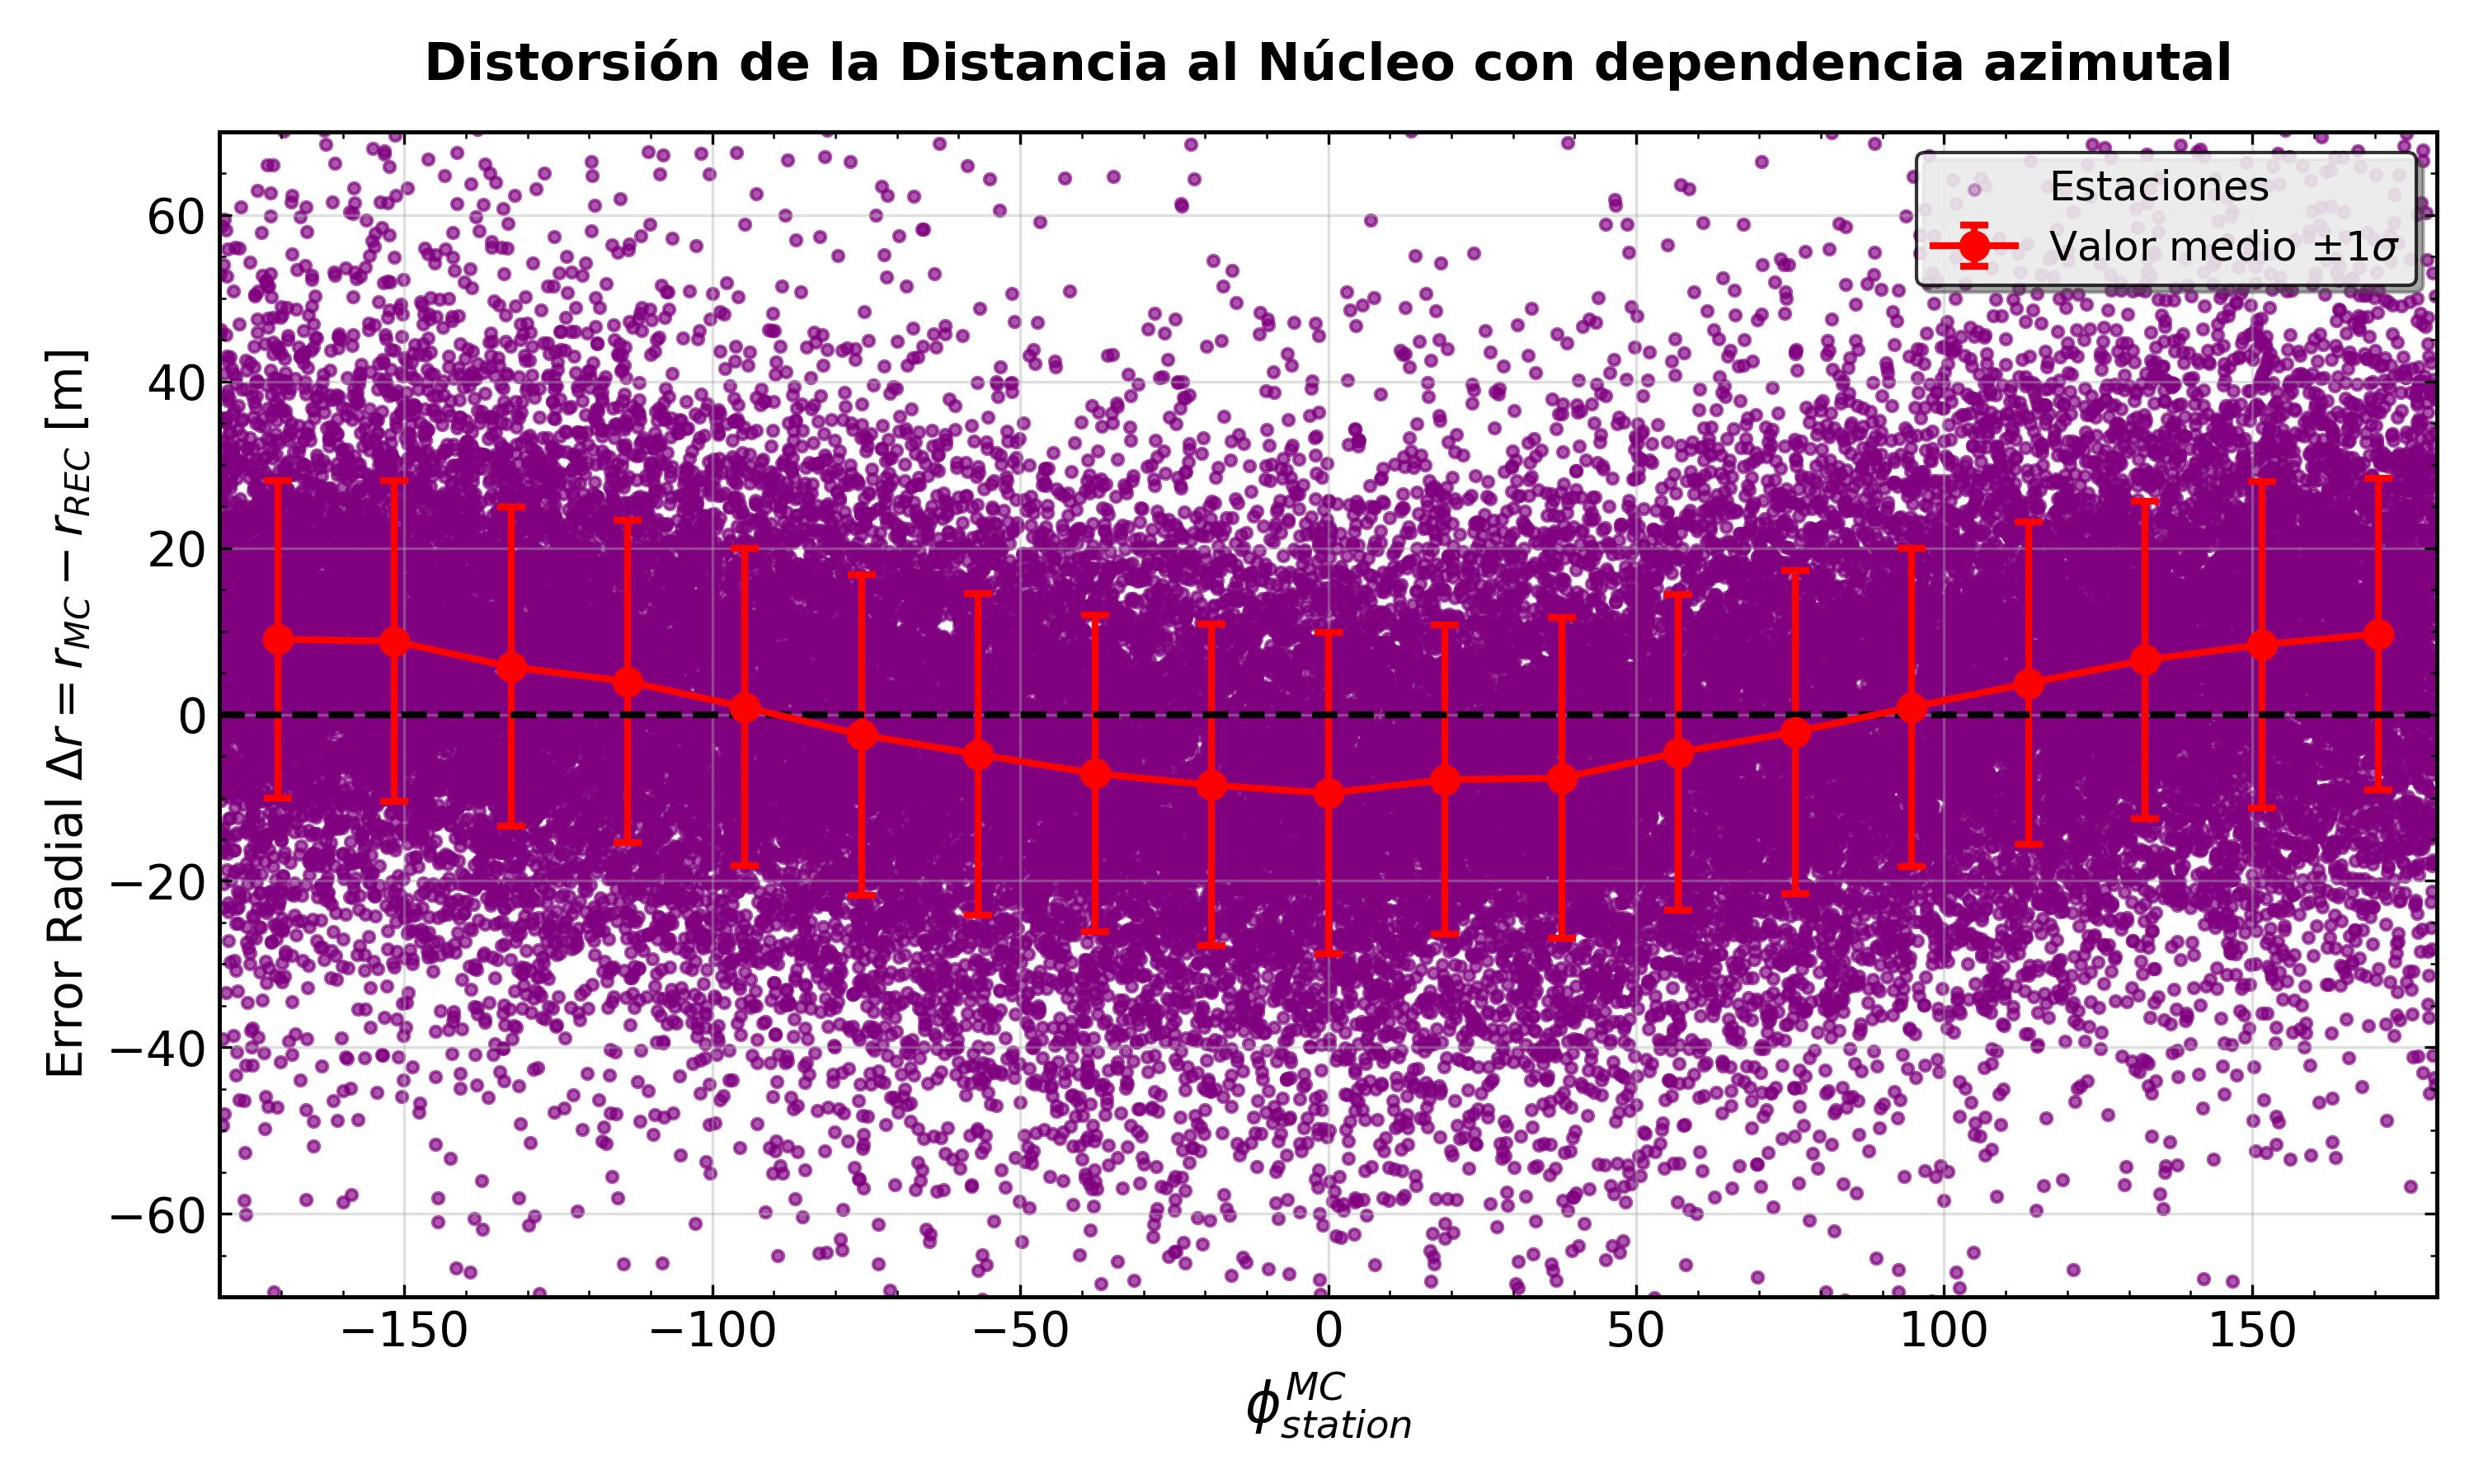
\includegraphics[width=1\textwidth]{capitulos/imagenes_capitulos/cap5/error_radial_azimut.jpg}
	\caption{Distorsión de la coordenada radial de las estaciones del \textit{Infill} en función del ángulo azimutal. La modulación armónica demuestra que el núcleo reconstruido no sufre un esparcimiento aleatorio, sino un corrimiento sistemático a lo largo del eje temprano-tardío.}
	\label{fig:bias_core_azimut}
\end{figure}

Una justificación física propuesta para explicar este comportamiento radica en la transición fenomenológica de la cascada y su conflicto intrínseco con la parametrización simétrica de la Función de Distribución Lateral (LDF). En el algoritmo de reconstrucción estándar la LDF, que se parametriza exculsivamente usando el SD, es asumida dependiente de la distancia radial pero estrictamente simétrica respecto del ángulo azimutal en el plano de la lluvia. A bajas inclinaciones, la fuerte atenuación de la abundante componente electromagnética genera asimetrías que son manejables dentro de los errores de resolución. Sin embargo, a medida que aumenta la inclinación cenital ($\theta \gtrsim 40^\circ$), la señal medida en superficie pasa a estar dominada por muones. Como se desarrollado, los muones de baja energía aumentan y se acumulan preferencialmente en la región tardía de la lluvia \cite{Cazon2012}. Esto genera una asimetría física real donde la zona tardía presenta un exceso espurio de densidad respecto a la zona temprana.

Es precisamente en este punto donde la imposición matemática del modelo simétrico falla sistemáticamente. Al intentar ajustar la posición del núcleo minimizando la función de costo, el algoritmo encuentra estaciones en la región tardía con un exceso anómalo de señal que su modelo simétrico no puede explicar si el núcleo estuviera en su posición verdadera. Dado que la LDF no contempla modulación azimutal, la única manera que tiene el ajustador para compensar esta discrepancia y lograr la convergencia es alterar la variable espacial: interpreta el exceso de señal como proximidad al eje de la cascada y la falta de señal como lejanía. Como consecuencia directa, el minimizador arrastra el núcleo reconstruido desde su posición real hacia la región tardía.

Este mecanismo explica la degradación de $A_1^{\mathrm{REC}}$ a altas inclinaciones que el \textit{Toy Model} de conteo no pudo replicar. El algoritmo \textit{Offline} impone un modelo simétrico sobre un fenómeno físicamente asimétrico (que se acentúa con el angulo cenital de la lluvia), logrando la convergencia al costo de absorber la asimetría de señal a través de un error de posición de las estaciones. Al evaluar la modulación armónica azimutal desde este núcleo reconstruido y desplazado, las estaciones tempranas quedan artificialmente más lejos de su posición relativa y las tardías artificialmente más cerca. La asimetría física es matemáticamente absorbida por el desplazamiento del núcleo, lavando la modulación azimutal y reduciendo de manera sistemática la amplitud $A_1$ observada en el UMD.

Este desplazamiento del núcleo impacta de manera crítica incluso a los datos del Anillo Denso, explicando la caída remanente del parámetro $A_1^{\mathrm{REC}}$ que el \textit{Toy Model} no pudo capturar. Aunque las estaciones del anillo virtual se sitúan a un radio de 450 m respecto al núcleo reconstruido, al estar dicho núcleo desplazado, el anillo resulta excéntrico respecto a la cascada real (MC). Esto introduce dos efectos acoplados que degradan la señal:

\begin{enumerate}
	\item \textbf{Lavado Azimutal:} Al calcular el ángulo en el plano de la lluvia desde un centro falso, el azimut asignado a cada estación difiere de su azimut físico real, mezclando de manera cruzada las señales de zonas de alta y baja densidad en el ajuste armónico.
	\item \textbf{Retroalimentación en el Conteo de Muones:} Los algoritmos del UMD que convierten las trazas de deposición de energía a número de muones reconstruidos dependen fuertemente de la geometría de incidencia de la partícula. Al suministrarse parámetros geométricos erróneos (distancias y ángulos falsos derivados del núcleo desplazado), la reconstrucción del UMD impone sesgos no lineales. Sistemáticamente se subsamplean muones en la región temprana y se sobreestiman en la tardía para forzar la compatibilidad con el modelo de LDF asimétrico, consolidando la degradación de la asimetría de atenuación original.
\end{enumerate}

En síntesis, la imposición de una LDF simétrica sobre lluvias físicamente asimétricas induce un corrimiento del núcleo que corrompe tanto la posición angular como la reconstrucción local de la señal. Esto demuestra que la asimetría física observada a nivel Monte Carlo es suprimida algorítmicamente durante la reconstrucción \textit{Offline}, lo que explica la caída de amplitud reportada a niveles de altas inclinaciones.

\subsection{Estudios de Robustez}
\label{subsec:robustez}

Se estudio también el comportamiento del detector y el parámetro de asimetría, al enfrentarse a situaciones en las que, al ser circunstancia donde la física es la misma especialmente considerando los efectos de la atenuación atmosférica, no se espera ver cambios en su performance.

\subsubsection{Invariancia azimutal de incidencia ($\phi_{shower}$)}
\label{subsubsec:invariancia_phi}

Para asegurar que la asimetría medida sea una propiedad intrínseca de la cascada y no un artefacto de la orientación del arreglo, se evaluó la estabilidad de $A_1$ en función del ángulo azimutal de entrada de la lluvia ($\phi_{\text{shower}}$). Para esto se separaron los datos del anillo denso en 6 bines equiespaciados en función del angulo de incidencia de la lluvia y se repitio el análisis explicando en la sección \ref{subsec:entorno_control} para cada uno de ellos.

 \begin{figure}[H]
	\centering
	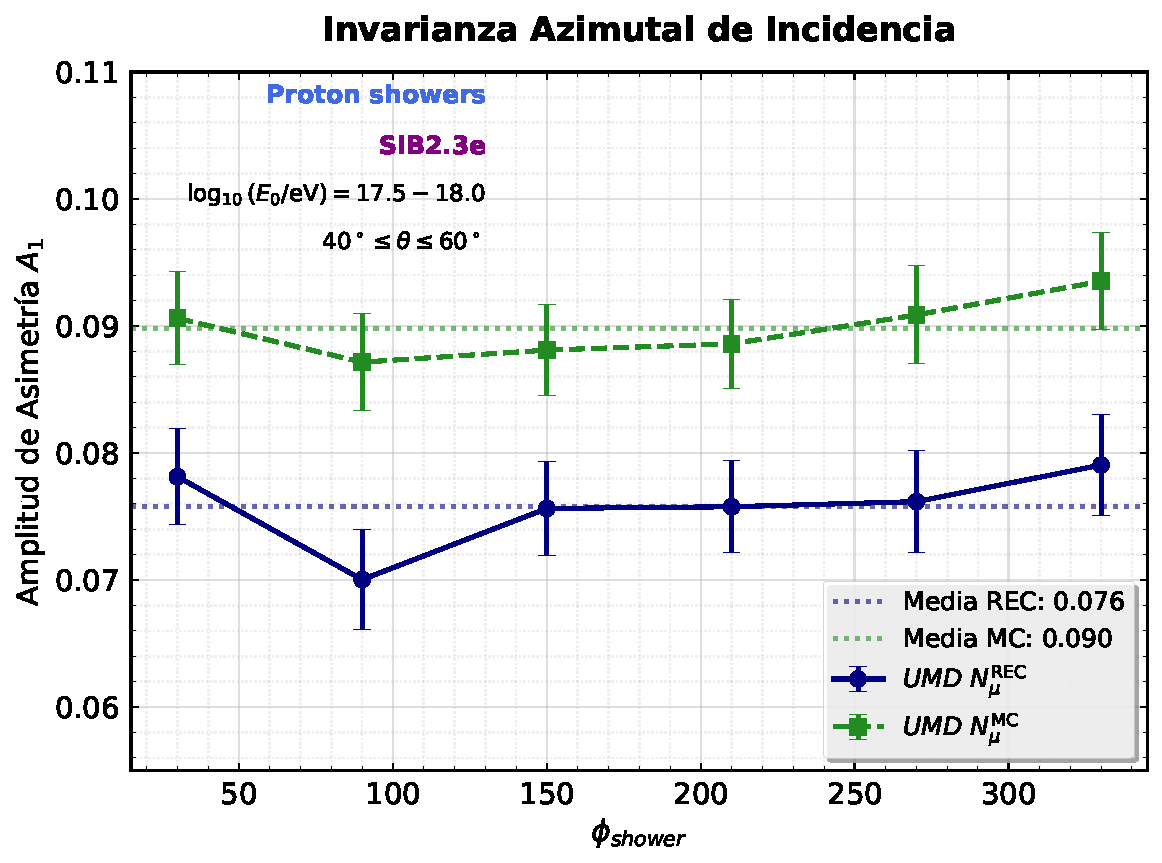
\includegraphics[width=1\textwidth]{capitulos/imagenes_capitulos/cap5/DenseRing_Systematics_Isotropy.pdf}
	\caption{Amplitud $A_1$ en función del ángulo azimutal de la lluvia. Se observa la independencia del observable respecto a la dirección de arribo.}
	\label{fig:robustez_phi}
 \end{figure}

En la Figura \ref{fig:robustez_phi} se analizo el dataset de protones con el modelo \texttt{Sibyll 2.3e} para lluvias inclinadas ($40^\circ < \theta < 60^\circ$). Se ve que el valor ajustado del parametro de asimetría $A_1$ no depende del angulo de incidencia de la lluvia, como era esperado. Esto es una buena prueba de estrés para los fundamentos del trabajo y que garantiza que se puede avanzar en el análisis en pos de hacer discriminacion de masa. Nuevamente aparece la discrepancia entre los valores absolutos de asimetria usando los muones inyectados y los reconstruidos.

\subsubsection{Independencia del modelo hadrónico}
\label{subsubsec:independencia_modelo}

Análogamente, se evaluó la robustez de la asimetría $A_1$ frente al uso de diferentes modelos de interacciones hadrónicas en las simulaciones. Para ello, se comparó la evolución del parámetro $A_1$ para un mismo primario (Helio) y rango de energía utilizando diferentes librerías fenomenológicas. Dada la disponibilidad de datos detallada en el Capítulo 4, se contrastaron las cascadas simuladas con los modelos \texttt{SIBYLL 2.3e} y \texttt{QGSJet-III.01}.

Aunque no existe garantía teórica de que ambos modelos predigan densidades totales de muones idénticas (debido a las diferencias en el déficit muónico intrínseco de cada parametrización), la modulación relativa $A_1$ debería presentar una consistencia cualitativa. Confirmar esta independencia es fundamental para validar el uso de la asimetría en la discriminación de masa y justificar la potencial combinación de conjuntos de datos para incrementar la estadística. 

Para llevar a cabo esta validación, se replicó el análisis angular realizando ajustes independientes por bin cenital, tal como se detalló en la sección \ref{subsec:entorno_control}. A su vez, se calculó la diferencia relativa porcentual entre los valores de amplitud obtenidos por ambos modelos, propagando las incertezas estadísticas correspondientes. La comparación de estas distribuciones se presenta en la Figura \ref{fig:modelos_hadronicos}.

\begin{figure}[H]
	\centering
	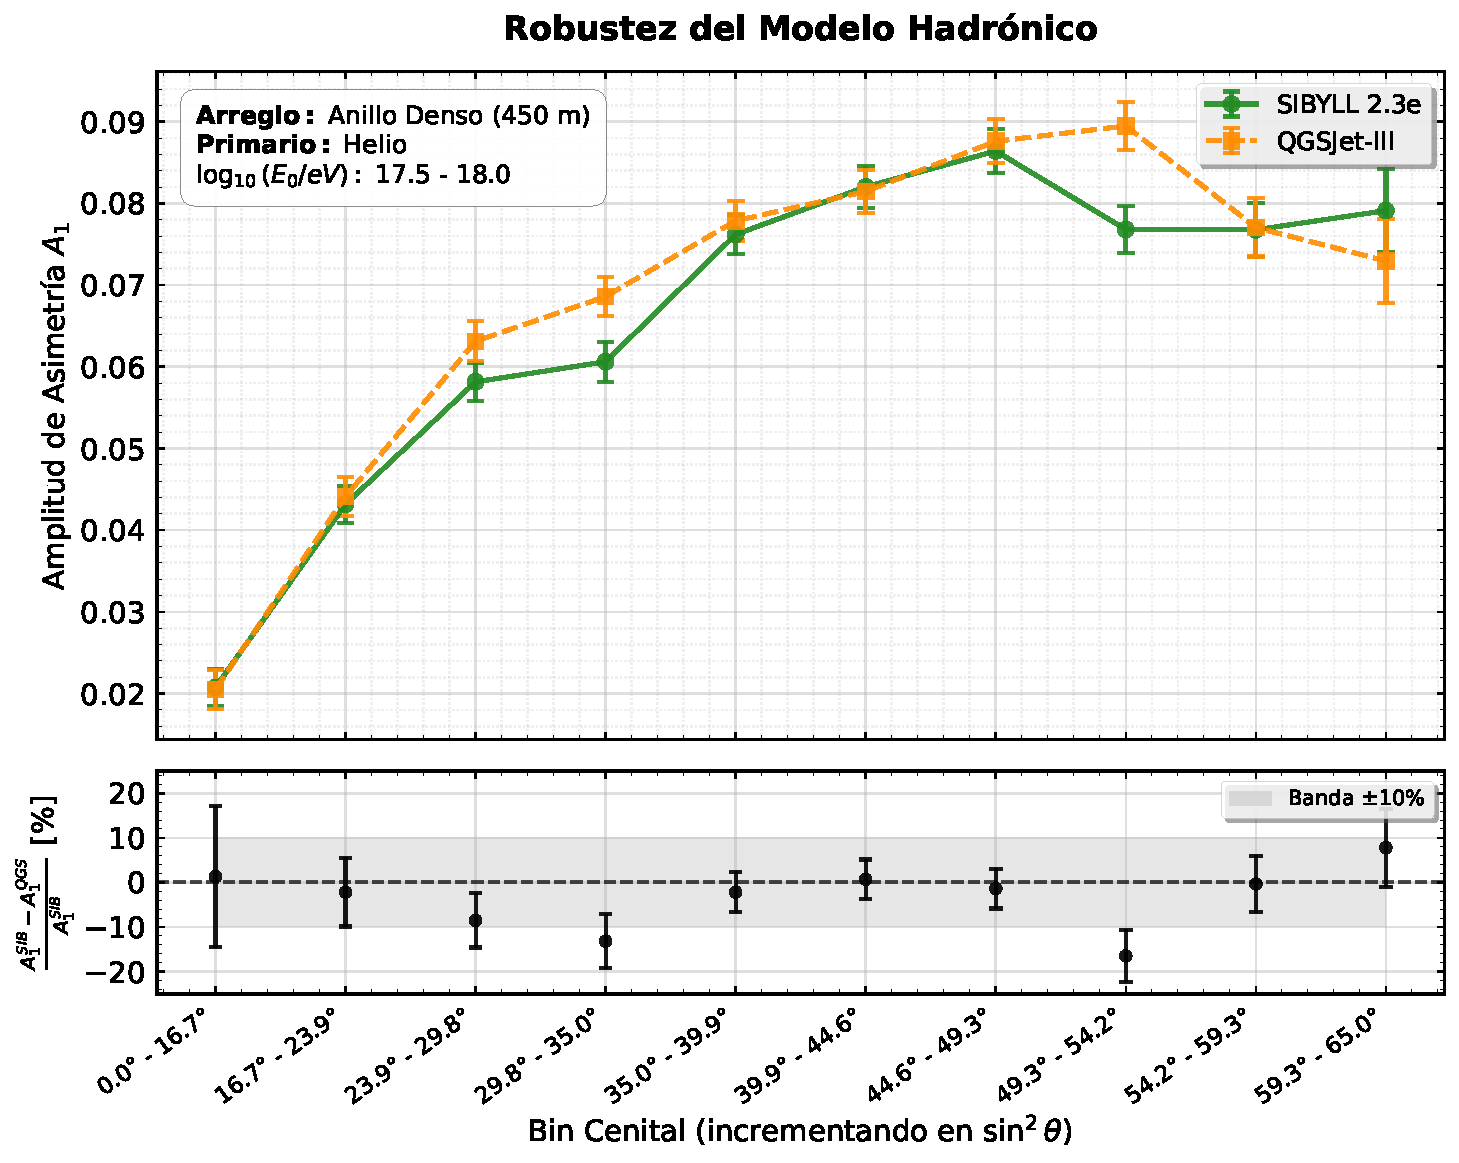
\includegraphics[width=1\textwidth]{capitulos/imagenes_capitulos/cap5/Hadronic_Uncertainty_Helium.pdf}
	\caption{Comparación de la amplitud $A_1$ para lluvias de Helio simuladas con diferentes modelos hadrónicos. El panel inferior muestra que la diferencia relativa se mantiene mayoritariamente dentro de una banda de tolerancia aceptable, indicando una tendencia común independiente del modelo.}
	\label{fig:modelos_hadronicos}
\end{figure}

Como se observa en el panel superior, la evolución de la asimetría presenta una consistencia morfológica excelente entre ambos modelos a lo largo de todo el rango angular. El panel inferior cuantifica esta concordancia: la diferencia relativa se mantiene predominantemente dentro de una banda de tolerancia del $\pm 10\%$, con desviaciones estadísticas puntuales que no superan el $15\%$. Este resultado confirma empíricamente que la amplitud de la asimetría azimutal $A_1$ es un observable robusto. Su forma funcional y magnitud relativa están dominadas por la cinemática macroscópica de la cascada y la atenuación atmosférica, manteniéndose esencialmente invariantes frente a los detalles microscópicos del modelo de interacción hadrónica empleado por el generador de Monte Carlo.

\subsection{Dependencia de la amplitud $A_1$ con la energía del primario}
\label{subsec:dependencia_energia}

Para evaluar la estabilidad del observable frente a variaciones cinemáticas, se analizó la evolución del parámetro de asimetría $A_1$ en función de la energía del rayo cósmico primario dentro de la banda de interés, $\log_{10}(E/\mathrm{eV}) \in [17.5, 18.0]$. Utilizando el conjunto de simulaciones de protones (\texttt{SIBYLL 2.3e}) restringido al rango angular de mayor desarrollo de asimetría ($40^\circ \leq \theta \leq 60^\circ$), los datos se particionaron en 5 bines de energía reconstruida. Los resultados de los ajustes armónicos para cada intervalo se presentan en la Figura \ref{fig:a1_vs_energia}.

\begin{figure}[H]
	\centering
	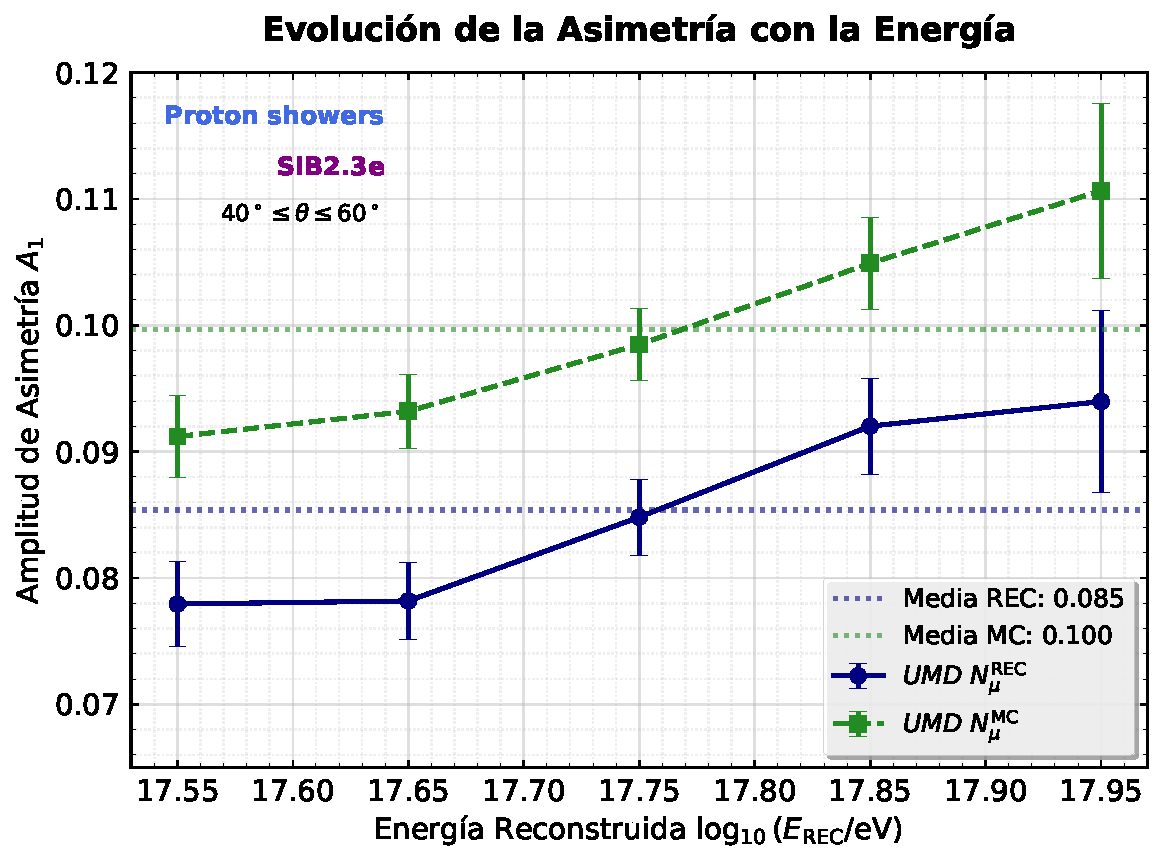
\includegraphics[width=1\textwidth]{capitulos/imagenes_capitulos/cap5/DenseRing_Systematics_Energy.pdf}
	\caption{Evolución de la amplitud de asimetría $A_1$ en función de la energía reconstruida para cascadas de protón simuladas con \texttt{SIBYLL 2.3e}. Se observa un leve incremento lineal en la asimetría a mayores energías, presente tanto a nivel Monte Carlo como en la reconstrucción.}
	\label{fig:a1_vs_energia}
\end{figure}

A priori, al tratarse de un rango energético relativamente estrecho (media década logarítmica), no se esperaba observar una fuerte dependencia funcional. Sin embargo, los resultados revelan un leve pero sistemático incremento lineal de la amplitud $A_1$ a medida que aumenta la energía, comportamiento que es capturado consistentemente tanto por los datos ideales (MC) como por los reconstruidos (REC).

La hipótesis de trabajo propuesta para explicar este comportamiento físico radica en el corrimiento de la profundidad del máximo de desarrollo de la cascada ($X_{\mathrm{max}}$). Teóricamente, un aumento en la energía del primario implica que la lluvia penetra más profundamente en la atmósfera antes de alcanzar su número máximo de partículas, acercando el $X_{\mathrm{max}}$ al nivel del suelo. Al reducirse la distancia atmosférica remanente entre el máximo de la lluvia y los detectores, la cascada observada resulta longitudinalmente más 'joven'. Esto altera los gradientes de densidad de partículas a través del plano de la lluvia, impactando directamente en la magnitud de la asimetría de atenuación. Cabe destacar que, si bien esta interpretación fenomenológica vincula lógicamente el incremento de $A_1$ con la evolución del $X_{\mathrm{max}}$, en el marco de este trabajo constituye una hipótesis interpretativa que sienta las bases para futuros estudios dedicados a correlacionar el desarrollo longitudinal con la topología en superficie.

Desde el punto de vista metodológico, el hallazgo más relevante de este escrutinio es la escala de la variación. Si bien la dependencia con la energía existe, la variación absoluta del parámetro a lo largo de toda la década es marginal ($\Delta A_1 \approx 0.015$). Esta estabilidad garantiza que la integración de todos los eventos del rango $\log_{10}(E/\mathrm{eV}) \in [17.5, 18.0]$ no inducirá un lavado ni ensanchará significativamente las distribuciones de manera crítica. Por consiguiente, queda plenamente justificado realizar el estudio de discriminación de masa primaria utilizando el \textit{dataset} completo de forma integrada, lo cual resulta imperativo para maximizar el poder estadístico sin comprometer la sensibilidad del observable.

\subsection{Discriminación de Masa Primaria: Protón vs. Hierro}
\label{sec:discriminacion_masa}

Habiendo caracterizado los efectos sistemáticos y validado la estabilidad de la reconstrucción en el entorno del Anillo Denso, el objetivo culminante de este análisis es evaluar la capacidad del observable $A_1$ para discriminar la naturaleza química del rayo cósmico primario. Para ello, se compararon las distribuciones de amplitud de asimetría para las poblaciones extremas de masa: primarios livianos (protones) y primarios pesados (hierro, conformados por 56 protones). 

Al evaluar el parámetro $A_1$ para ambos conjuntos de datos con energías $\log_{10}(E/\mathrm{eV}) \in [17.5, 18.0]$ usando el modelo hadrónico \texttt{Sibyll 2.3e}, se observó una separación sistemática entre las curvas. La población de protones desarrolla amplitudes de asimetría consistentemente mayores a las correspondientes a la población de hierro a lo largo del rango angular evaluado para la mayoría de los bines.

\subsubsection{El Factor de Mérito ($MF$) y el \textit{Sweet Spot} de discriminación}
\label{subsec:sweet_spot}

Para cuantificar rigurosamente el poder separador del observable, es necesario evaluar no solo la distancia entre los valores medios de ambas poblaciones, sino también su dispersión estadística. Con este fin, se utilizo como métrica de evaluación el Factor de Mérito ($MF$) como:

\begin{equation}
	MF = \frac{|\langle A_1^{\text{P}} \rangle - \langle A_1^{\text{Fe}} \rangle|}{\sqrt{(\sigma_{A_1}^{\text{P}})^2 + (\sigma_{A_1}^{\text{Fe}})^2}}
\end{equation}

Donde $\langle A_1 \rangle$ y $\sigma_{A_1}$ representan el valor medio y la desviación estándar de la amplitud de asimetría ajustada para cada primario. Un valor de $MF > 1$ indica un régimen donde la separación entre las distribuciones supera a sus anchos característicos, permitiendo una discriminación estadística robusta. En la Figura \ref{fig:mf_sweet_spot} se presenta la evolución del Factor de Mérito en función del ángulo cenital de la cascada.

El análisis de esta figura revela un comportamiento fuertemente dependiente de la inclinación. Se identifica de manera clara una región óptima, o \textit{Sweet Spot} de discriminación, en el rango angular $40^\circ \leq \theta \leq 55^\circ$. En esta ventana, el $MF$ alcanza valores máximos del orden de $\approx 2.5$, garantizando la excelente capacidad de la amplitud de asimetría para hacer separación de masas.

\begin{figure}[H]
	\centering
	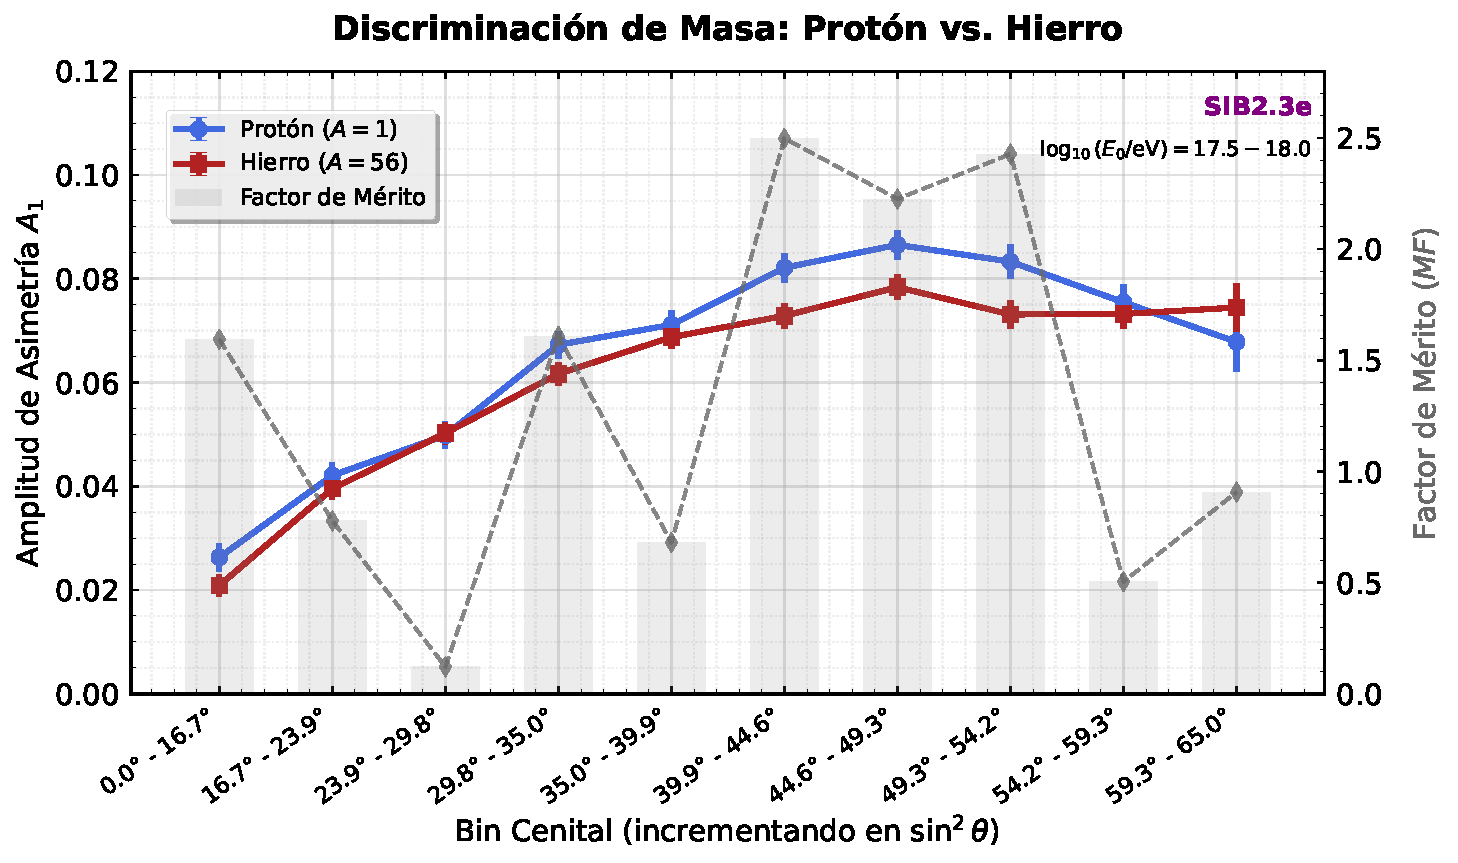
\includegraphics[width=1\textwidth]{capitulos/imagenes_capitulos/cap5/Mass_Discrimination_MF.pdf}
	\caption{Evolución del Factor de Mérito ($MF$) en función del ángulo cenital. Se identifica un \textit{Sweet Spot} de máxima separación entre bines de $40^\circ$ y $55^\circ$, donde el poder de discriminación alcanza su máximo antes de degradarse por efectos instrumentales.}
	\label{fig:mf_sweet_spot}
\end{figure}

Fuera de este rango, el poder de discriminación decae abruptamente o se vuelve inestable debido a dos regímenes limitantes de carácter completamente distinto:

\begin{enumerate}
	\item \textbf{Régimen de baja inclinación ($\theta < 35^\circ$):} En cascadas cuasi-verticales, la diferencia de camino atravesado por las partículas entre la región temprana y tardía es mínima. Por lo tanto, la asimetría de atenuación física es en modulo tan pequeña que la diferencia absoluta entre protón y hierro resulta imperceptible, quedando enmascarada por las fluctuaciones estadísticas propias de la lluvia.
	\item \textbf{Régimen de alta inclinación ($\theta > 60^\circ$):} Aunque a estos ángulos la asimetría física debería ser máxima, entra en juego el colapso de la reconstrucción instrumental. Tal como se demostró exhaustivamente en la Sección \ref{subsec:mc_vs_rec}, a grandes inclinaciones el ajustador \textit{Offline} induce un corrimiento sistemático del núcleo, entre otros problemas. Este sesgo geométrico genera un lavado azimutal y un sobreconteo direccional de muones que distorsiona la asimetría. Este efecto no solo achata artificialmente las medias de $A_1$, reduciendo el numerador del $MF$, sino que introduce un ruido correlacionado masivo que dispara el tamaño de las desviaciones estándar ($\sigma$), destruyendo por completo la capacidad discriminatoria del detector en este régimen.
\end{enumerate}

\subsection{Interpretación Física: dependencia con el $X_{max}$}
\label{subsec:interpretacion_fisica}

La existencia de una separación sistemática donde $\langle A_1^{\text{P}} \rangle > \langle A_1^{\text{Fe}} \rangle$ no es un resultado estadístico aislado, sino la manifestación en superficie de la evolución longitudinal intrínseca de la cascada atmosférica. La hipótesis de trabajo que actúa como justificación física de este fenómeno radica en la dependencia de la asimetría azimutal con la profundidad atmosférica del máximo desarrollo de la lluvia ($X_{\text{max}}$), de manera análoga al análisis realizado en la Sección \ref{subsec:dependencia_energia} respecto a la energía del primario.

Este comportamiento encuentra su marco teórico en el Modelo de Superposición y el modelo de Heitler-Matthews para cascadas hadrónicas \cite{matthews2005}. Según este esquema, una cascada iniciada por un núcleo \textbf{pesado} de masa $A$ y energía total $E_0$ se comporta estadísticamente como la superposición de $A$ sub-cascadas nucleónicas independientes, cada una portando una fracción de energía $E_0/A$. Dado que la sección eficaz de interacción crece con el tamaño del núcleo, y la energía por nucleón es sustancialmente menor, las cascadas de hierro ($A=56$) interactúan mucho más alto en la atmósfera que las de protón ($A=1$). Como resultado directo, agotan su desarrollo longitudinal prematuramente, situando el $X_{\text{max}}$ de una lluvia de hierro a una profundidad atmosférica significativamente menor (mayor altitud geográfica) comparado con las lluvias de protones. 

Esta separación en la profundidad de máximo desarrollo entre especies primarias es un fenómeno empíricamente robusto, medido de forma extensiva por los telescopios de fluorescencia del Observatorio Pierre Auger \cite{yushkov2019mass}. En la Figura \ref{fig:auger_xmax} se ilustra esta dependencia, evidenciando cómo el $X_{\text{max}}$ se ubica más profundo a mayores energías y cómo los primarios livianos penetran sistemáticamente más que los pesados.

\begin{figure}[H]
	\centering
	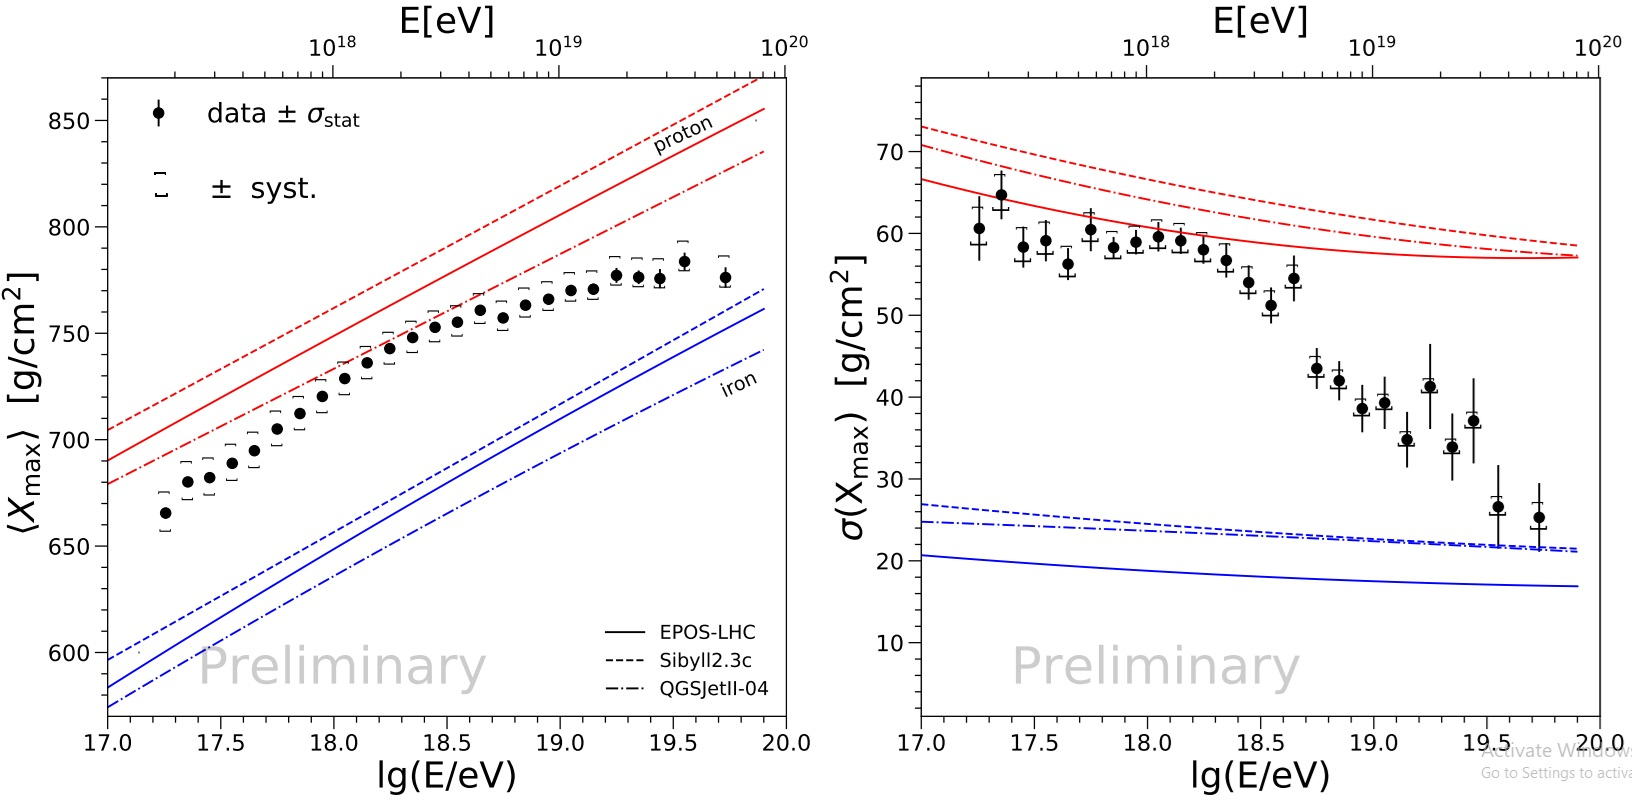
\includegraphics[width=1\textwidth]{capitulos/imagenes_capitulos/cap5/x_max.jpg}
	\caption{Evolución del valor medio de $X_{\text{max}}$ (izquierda) y sus fluctuaciones (derecha) en función de la energía primaria, medido por el Observatorio Pierre Auger. Se observan las curvas teóricas de los modelos hadrónicos acotando el comportamiento entre protón (líneas rojas superiores) y hierro (líneas azules inferiores). Se ve también la dependencia lineal que hay entre el $X_{max}$ y el logaritmo de la energia del primario. Extraído de \cite{yushkov2019mass}.}
	\label{fig:auger_xmax}
\end{figure}

Para comprender por qué esta diferencia en la profundidad del máximo impacta directamente sobre la amplitud de asimetría $A_{1}$ medida en superficie, es necesario analizar la dinámica del desarrollo longitudinal y su proyección topológica sobre el arreglo.

\begin{figure}[H]
	\centering
	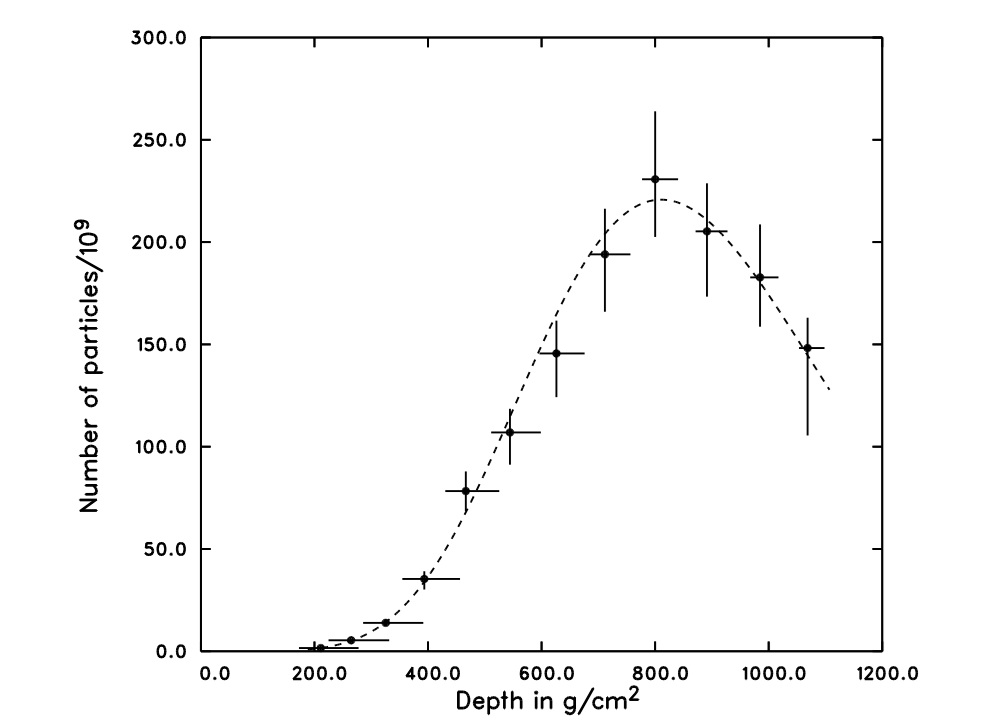
\includegraphics[width=1\textwidth]{capitulos/imagenes_capitulos/cap5/ammount_xmax.jpg}
	\caption{El gráfico corresponde al evento de mayor energía detectado por el experimento Fly's Eye ($E \approx 3.2 \times 10^{20}$ eV) extraído de \cite{FlysEye1995}. Se observa claramente la fase de multiplicación hasta alcanzar la profundidad del máximo, seguida de la atenuación de la cascada. La distancia recorrida de atmosfera hasta llegar al máximo es lo que se denomina $X_{max}$.}
	\label{fig:longitudinal_profile}
\end{figure}

Como se ve en la Figura \ref{fig:longitudinal_profile} a medida que la lluvia penetra en la atmósfera, experimenta una fase de multiplicación en avalancha hasta alcanzar la profundidad del máximo, $X_{max}$. Superado este umbral, la energía media de las partículas secundarias cae por debajo de la energía crítica para seguir alimentando la creación de nuevas partículas, momento en el cual los procesos de pérdida por ionización y el decaimiento dominan sobre la sección eficaz de interacción, forzando a la cascada a entrar en su fase de atenuación.

Dado que el UMD es un detector subterráneo, ciego a la componente electromagnética, la asimetría registrada debe depender estrictamente del historial de producción y transporte de la componente muónica. Los muones se originan principalmente a partir del decaimiento de mesones cargados (piones y kaones, ej. $\pi^{\pm} \rightarrow \mu^{\pm} + \nu_{\mu}$). La tasa de producción de estas partículas sigue de cerca el perfil longitudinal del cascada hadrónica y alcanza su propio máximo, denominado $X_{max}^{\mu}$, a una profundidad muy similar al $X_{max}$ \cite{Cazon2012}.

La modulación azimutal remanente en esta componente muónica está gobernada  fundamentalmente por un efecto de proyección geométrica acoplado a la divergencia angular de las partículas. Sea $D$ la distancia que recorren las partículas, medida a lo largo del eje de la lluvia, desde la región de máxima producción muónica ($X_{max}^{\mu}$) hasta el centro del arreglo de detectores en el suelo. Al incidir una cascada inclinada con ángulo cenital $\theta$, la porción del frente de partículas que impacta en la región tardía debe recorrer una distancia geométrica adicional $\Delta d$ respecto a las partículas que impactan en la región temprana, para un mismo radio $r$ en el plano de la lluvia.

Dado que la densidad de partículas provenientes de un haz colimado decae radialmente como la divergencia espacial  $\propto 1/d^2$ \cite{Cazon2012}, la magnitud de la asimetría temprano-tardía producida por este efecto depende fuertemente del cociente entre la diferencia de camino y la distancia total de propagación $\Delta d / D$.

Cuando una lluvia inducida por un núcleo de Hierro impacta contra el arreglo, el observador percibe una cascada en un estado longitudinal maduro. Debido a que su $X_{max}$ se encuentra a bajas profundidades atmosféricas (altas altitudes geográficas), la distancia geométrica $D$ desde el punto de producción hasta el suelo es inmensa. En consecuencia, el camino extra $\Delta d$ requerido para alcanzar la región tardía representa una fracción marginal del trayecto total ($\Delta d / D \ll 1$). Ademas tras recorrer decenas de kilómetros, la dispersión cinemática intrínseca y la deflexión geomagnética homogenizan las trayectorias de los muones, mitigando las diferencias bruscas y resultando en una distribución azimutalmente uniforme, lo que se traduce en un valor de $A_1$ comparativamente bajo.

En contraste, los primarios livianos (Protones) penetran profundamente en la atmósfera, situando su $X_{max}$ mucho más próximo a la superficie topográfica. Esta proximidad reduce severamente la distancia $D$, incrementando significativamente el peso relativo de la dispersión espacial ($\Delta d / D$). Para frentes de cascada ubicados cerca del punto de observación, la atenuación longitudinal castigan asimétricamente a la región tardía frente a la región temprana generado un valor de asimetría mayor.

En conclusión, la profundidad de penetración del primario modula la agudeza topológica de la cascada medida en tierra. Las lluvias con un $X_{max}$ profundo (protones o lluvias de mayor energía) exponen al UMD a frentes de partículas más concentrados espacialmente, donde cualquier diferencia de proyección geométrica induce fluctuaciones grandes en las densidades relativas de muones. Este mecanismo fenomenológico consolida a la amplitud de asimetría $A_1$ no solo como un descriptor morfológico de la LDF, sino como un trazador valioso de la evolución longitudinal y, en última instancia, como un instrumento extra para realizar discriminación de la masa $A$ del rayo cósmico primario.

\subsubsection{Contraste fenomenológico con el Detector de Superficie}
\label{subsec:contraste_sd_bradfield}

El comportamiento de la asimetría azimutal ha sido desarrollado en detalle en el trabajo de Bradfield \cite{BradfieldThesis} aplicado a las señales del Detector de Superficie (SD). Es pertinente contextualizar los resultados obtenidos con el UMD frente a dichos estudios para evidenciar la naturaleza divergente de las componentes de la cascada.

Al analizar la dependencia de la asimetría con la evolución longitudinal de la cascada, surge una discrepancia física fundamental. En los análisis realizados sobre el SD, se reporta que la magnitud de la asimetría experimenta un decrecimiento a medida que aumenta la profundidad del máximo ($X_{max}$). Este comportamiento es directamente opuesto a la dinámica observada empíricamente en el UMD en las simulaciones, donde frentes de cascada más profundos (primarios livianos o de mayor energía) inducen una mayor amplitud $A_1$.

Esta aparente contradicción se puede explicar al considerar los regímenes físicos fundamentalmente distintos que dominan la propagación de cada componente atmosférica. La asimetría medida por el SD está gobernada de manera abrumadora por la componente electromagnética ($e^\pm, \gamma$). Como fue formalizado por Dova \textit{et al.} \cite{dova2003}, la asimetría de esta componente surge de la variación azimutal en el espesor atmosférico atravesado. Al propagarse en un régimen de rápida atenuación, la amplitud de la asimetría resulta proporcional al gradiente local de la curva de desarrollo longitudinal de la cascada:

\begin{equation}
	A_{EM} \propto \frac{1}{\rho_{EM}} \frac{\partial \rho_{EM}}{\partial X} \Delta X
	\label{eq:asym_em_taylor}
\end{equation}

Para las cascadas típicas observadas en Auger, el nivel del suelo se encuentra a una profundidad mayor que $X_{max}$, situando a los detectores en la fase de decaimiento de la curva de desarrollo. A medida que $X_{max}$ aumenta y la lluvia penetra más en la atmósfera, el punto de observación se aproxima al máximo de la cascada. En esta región de la curva de Gaisser-Hillas, la pendiente de atenuación es significativamente más suave (el gradiente $\partial \rho_{EM} / \partial X$ tiende a cero). Al desvanecerse este gradiente, la diferencia neta de densidad entre las regiones temprana y tardía inducida por el $\Delta X$ se suprime, lo que provoca el colapso sistemático de la asimetría observada en el SD reportado en \cite{BradfieldThesis}.

En estricto contraste, el UMD registra de manera pura la componente muónica. Tal como fue establecido inicialmente por Billoir \cite{GAP2000_017} y expandido en los modelos de Ave \textit{et al.} \cite{ave2017}, los muones de alta energía poseen una propagación cuasi-rectilínea y su distribución responde a la distancia geométrica al punto de producción en lugar del espesor atmosférico. Consecuentemente, su modulación azimutal es un efecto cinemático derivado de la divergencia del flujo de partículas, donde la densidad en el suelo decae con la inversa del cuadrado de la distancia ($\rho_\mu \propto 1/d^2$). 

Para una lluvia cuyo centro se produce a una distancia $D$ sobre el eje, un detector ubicado a un radio $r$ en el suelo se encuentra a una distancia efectiva $d \approx D - r \sin\theta \cos\phi$ respecto a la fuente, debido a la inclinación del frente. Aplicando una expansión de Taylor de primer orden (válida para $r \ll D$), la densidad angular resulta:

\begin{equation}
	\rho(\phi) \propto \frac{1}{(D - r \sin\theta \cos\phi)^2} \approx \frac{1}{D^2} \left( 1 + 2 \frac{r \sin\theta}{D} \cos\phi \right)
\end{equation}

Comparando esta expresión con la parametrización armónica estándar $\rho(\phi) = \rho_0 (1 + A_1 \cos\phi)$, se deriva directamente que la asimetría muónica depende de la inversa de la distancia de producción:

\begin{equation}
	A_{\mu} \approx 2 \frac{r \sin\theta}{D}
	\label{eq:asym_mu_cinematica}
\end{equation}

Un evento con un $X_{max}$ profundo implica que el rayo cósmico ha penetrado más en la atmósfera, situando el punto de producción muónica significativamente más cerca de los detectores. Esta proximidad reduce drásticamente el denominador $D$ en la Ec. \ref{eq:asym_mu_cinematica}. Al achicarse la distancia total de propagación, las diferencias espaciales relativas se magnifican, justificando el marcado incremento de la amplitud $A_1$ medido en el UMD para lluvias más penetrantes.

Finalmente, es crucial rediscutir la interpretación fenomenológica respecto a la composición primaria propuesta para el SD. Bradfield atribuye la menor asimetría del hierro respecto al protón, a igualdad de $X_{max}$, a su 'contenido adicional de muones'. Físicamente, la normalización absoluta de la componente muónica no altera la modulación relativa de su propia distribución. El origen de este corrimiento reside en el principio de superposición que ya se discutió en la sección \ref{subsec:interpretacion_fisica}. El SD mide una señal promediada ponderada por fracciones ($A^{SD} \approx f_{EM} A_{EM} + f_{\mu} A_{\mu}$). Como las lluvias inducidas por primarios pesados poseen una fracción de señal muónica ($f_{\mu}$) intrínsecamente mayor, el promedio del SD otorga más peso estadístico al término menos asimétrico ($A_{\mu}$), diluyendo la asimetría global observada. 

Esta caracterización cinemática demuestra que el SD constituye un observable de difícil interpretación para estudios de composición a través de la asimetría, debido a la supresión de su gradiente longitudinal cerca del máximo. En contrapartida, el UMD aísla un mecanismo estrictamente proyectivo regido por $1/D$, consolidándose como un instrumento robusto y físicamente transparente para estudiar el desarrollo de la lluvia.

\newpage

\clearpage
\setcounter{section}{5}
\phantomsection\label{review:06}
% !TEX root = ../main.tex

\section{Dinámica Radial del Arreglo \textit{Infill} en Simulaciones}
\label{cap:infill}

Habiendo validado la fenomenología de la asimetría azimutal en el entorno geométricamente controlado del Anillo Denso, se extendió el análisis a la topología real del arreglo de detectores pero aun utilizando simulaciones. A diferencia del Anillo Denso, el arreglo \textit{Infill} o arreglo regular de $750~m$, permite hacer un estudio sobre las estaciones de superficie y módulos enterrados reales, analizando el comportamiento de la asimetría en un espectro continuo de distancias al eje de la lluvia. Cabe destacar que, para mantener la coherencia con los estudios previos, la mayor parte del análisis desarrollado en esta sección utiliza exclusivamente la biblioteca de simulaciones de lluvias primarias de protones en el rango de energía de $\log_{10}(E/\mathrm{eV}) \in [17.5, 18.0]$.

Un objetivo central de esta etapa consistió en caracterizar el impacto de la reconstrucción instrumental sobre la preservación del observable $A_1$. Dado que en el entorno de simulaciones se tiene acceso simultáneo a la geometría verdadera de la lluvia (núcleo y ángulos Monte Carlo) y a su contraparte reconstruida, es posible evaluar el comportamiento del frente de partículas aislando la física subyacente de la degradación topográfica asociada a los errores sistematicos conocidos propios de la reconstrucción. En este capítulo se aborda cómo la dinámica de la cascada y la resolución del arreglo modulan la asimetría, marcando la transición desde un régimen de dominancia cinemática hacia uno de atenuación longitudinal.

\subsection{Arreglo \textit{Infill} usando el núcleo y ángulos Monte Carlo}
\label{subsec:infill_mc}

Para comprender la evolución intrínseca de la modulación azimutal, el análisis inicial se ejecutó forzando al \textit{pipeline} de procesamiento a utilizar las coordenadas del núcleo y la dirección de arribo extraídas directamente del nivel Monte Carlo. Esto permite estudiar la respuesta pura de los detectores sin el sesgo del difuminado espacial.

La fuerte dependencia radial y angular de los mecanismos que modulan la densidad de partículas exige una selección topográfica rigurosa. Por un lado, en la región radialmente cercana al centro de impacto ($r < 150$~m), la divergencia cinemática extrema descrita en la Sección \ref{subsubsec:divergencia} y el fuerte gradiente de la Función de Distribución Lateral (LDF) inducen fluctuaciones severas en la densidad. Promediar esta región junto con zonas más lejanas resulta contraproducente, ya que superpone regímenes fenomenológicos contradictorios. Por este motivo, se adoptó un bineado radial dinámico de $\Delta r = 150$~m, aplicando un corte fiducial que excluye dicho \textit{near-core}. 

Simultáneamente, para evitar la mezcla de zonas tempranas y tardías del frente de partículas que diluiría el valor medio de la señal, se particionó la fase azimutal en 12 intervalos ($\Delta\phi = 30^\circ$). Esta necesidad de mantener una alta pureza fenomenológica garantizando al mismo tiempo la robustez estadística en cada bin, definió también la segmentación del ángulo cenital en ventanas de $\Delta \theta = 10^\circ$ (con un intervalo final ampliado para lluvias muy inclinadas, $50^\circ \leq \theta < 65^\circ$). Las grillas completas con los datos junto a los ajustes armónicos y sus respectivos valores de $\chi^2/\text{ndf}$ en este espacio de fases se reportan en el Anexo \ref{anexo:ajustes_infill_mc}.

Al ajustar la densidad de muones registrada por el UMD a la función armónica como se describió en \ref{eq:ajuste_armonico}, se utilizó el estadístico de bondad de ajuste ($\chi^2/\text{ndf} \approx 1$) como métrica fundamental para validar las regiones con asimetría cuantificable. Esta convergencia estadística permite demostrar de manera contundente que, aislando correctamente las coronas radiales y angulares, la modulación azimutal muónica se describe a la perfección mediante un armónico de primer orden en ciertas regiones bien definidas, descartando la presencia de términos de orden superior.

En la Figura \ref{fig:a1_vs_r_theta_mc} se sintetizan los resultados de este barrido global, presentando la evolución de la amplitud de asimetría $A_1$ extraída para el UMD en función de la distancia al eje $r$ para las distintas inclinaciones.

\begin{figure}[H]
	\centering
	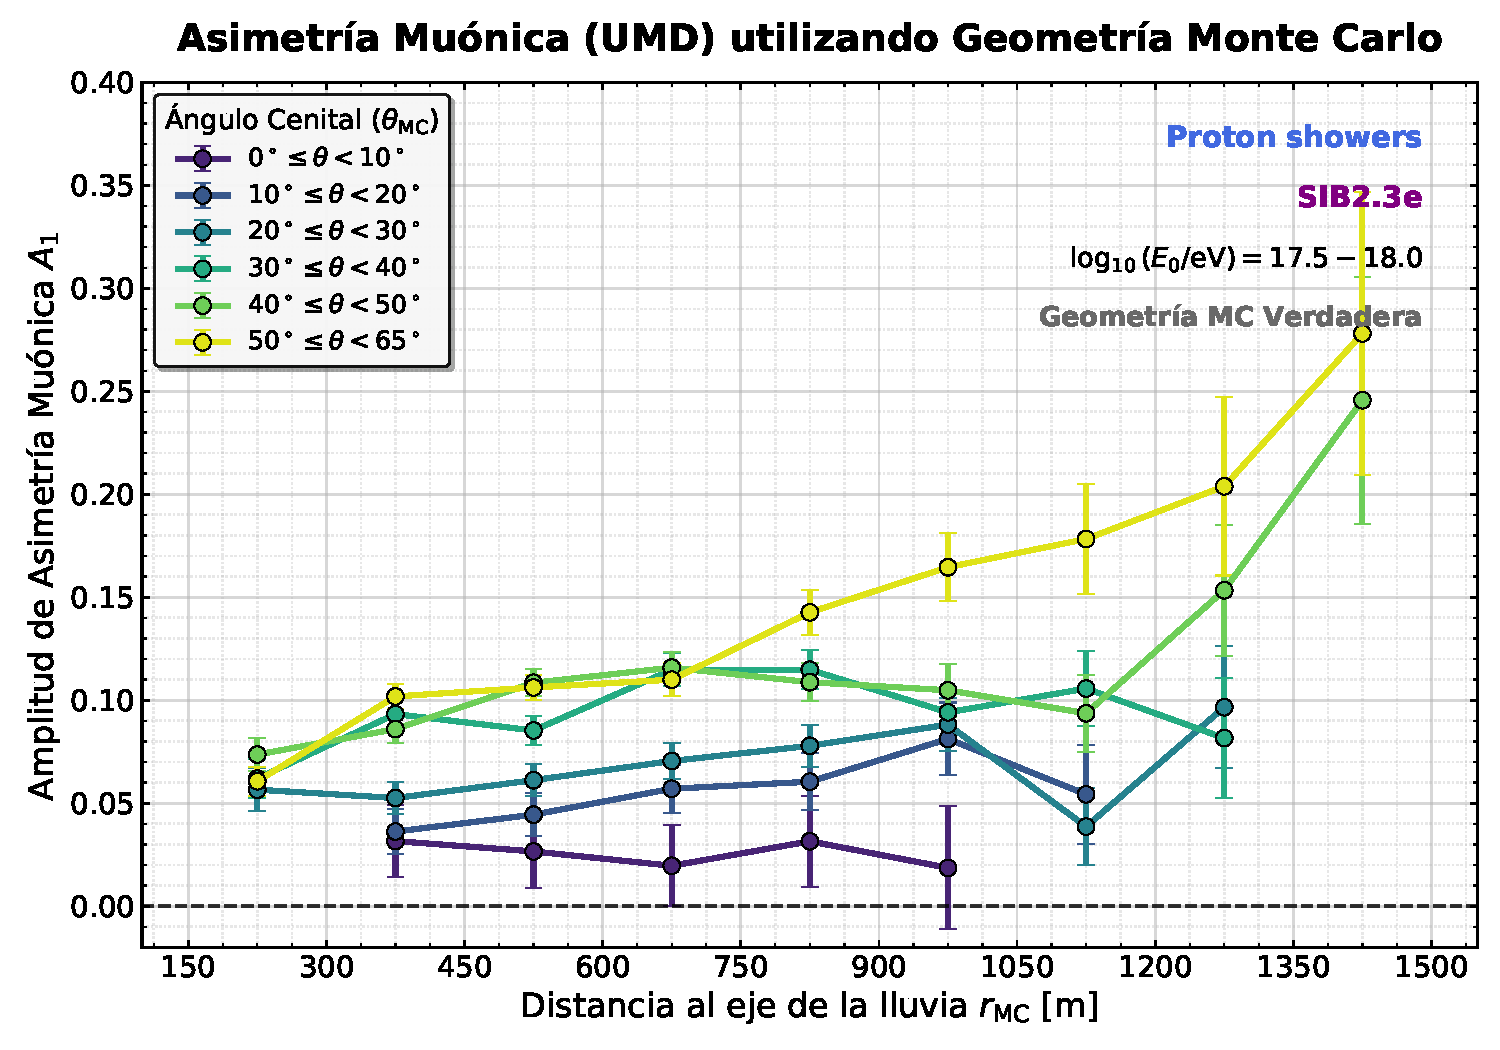
\includegraphics[width=1\textwidth]{capitulos/imagenes_capitulos/cap6/Global_A1_vs_R_Theta_MC.pdf}
	\caption{Evolución de la amplitud de asimetría $A_1$ en función de la distancia al núcleo para distintos rangos de inclinación cenital. El análisis utiliza la geometría verdadera (Monte Carlo) y un bineado radial dinámico ajustado a la viabilidad estadística de cada régimen.}
	\label{fig:a1_vs_r_theta_mc}
\end{figure}

El comportamiento observado confirma las predicciones del modelo de competencia cinemática-atenuación y revela los límites de viabilidad estadística del arreglo:

\begin{itemize}
	\item \textbf{Régimen Vertical ($0^\circ \leq \theta < 10^\circ$):} Como es esperable por simetría geométrica, las lluvias cuasi-verticales no exhiben una dirección temprana o tardía privilegiada frente a la atenuación atmosférica. La modulación azimutal es nula ($A_1 \approx 0$) a lo largo de todo el arreglo.
	
	\item \textbf{Régimen Intermedio ($10^\circ \leq \theta < 40^\circ$):} A medida que la lluvia se inclina, la diferencia de recorrido geométrico y la atenuación atmosférica transversal comienzan a romper la simetría. Para inclinaciones moderadas ($10^\circ - 30^\circ$), el observable $A_1$ adquiere valores positivos con un crecimiento de tendencia casi lineal. Sin embargo, a distancias del orden de $\sim 1100$~m, la densidad muónica decae drásticamente lo que se interpreta como causado por fluctuaciones de Poisson severas que parecen resolverse en el siguiente bin radial. Por su parte,en el siguiente bin angular cenital ($30^\circ - 40^\circ$), aparenta manifestarse un fenómeno de saturación o plateau: la asimetría crece rápidamente pero se estabiliza formando una meseta a partir de los $800$~m.
	
	\item \textbf{Régimen Inclinado ($40^\circ \leq \theta < 65^\circ$):} Para ángulos cenitales grandes, la cantidad de atmósfera atravesada por la cascada se incrementa drásticamente siguiendo la dependencia geométrica de la secante ($X \propto 1/\cos\theta$). El gradiente longitudinal se vuelve el mecanismo dominante absoluto de la cascada. A diferencia de los regímenes anteriores, el crecimiento de la amplitud $A_1$ es monótono y significativamente mayor, sin presentar saturación. En estas condiciones extremas, la enorme diferncia entre la densidad de partículas entre las regiones tempranas y tardias garantiza que la coherencia de la asimetría sea tan robusta que el ajuste sobreviva con alta fidelidad incluso en la periferia más lejana del arreglo \textit{Infill} ($1350 - 1500$~m).
\end{itemize}

Estos resultados demuestran que, en ausencia de incertezas geométricas instrumentales, la asimetría muónica es un observable altamente sensible a la evolución longitudinal de la cascada, estableciendo una cota teórica superior para lo que el UMD puede aspirar a medir en condiciones experimentales. Cabe destacar que el dominio radial evaluado no es uniforme, sino que ha sido adaptado a la cinemática de cada franja cenital. La extensión de las curvas fue delimitada aplicando un criterio de selección riguroso: el análisis se restringe exclusivamente a aquellas regiones donde la métrica de bondad de ajuste ($\chi^2/\text{ndf}$) y la inspección fenomenológica visual garantizan la robustez y fidelidad estadística del observable.

Es pertinente destacar que, al replicar este mismo análisis sustituyendo la cantidad de muones inyectada ($N_\mu^{\mathrm{MC}}$) por la cantidad reconstruida por el algoritmo del UMD ($N_\mu^{\mathrm{REC}}$), pero manteniendo el núcleo y los ángulos Monte Carlo, la fenomenología global se conserva de forma idéntica. Como se ilustra en la Figura \ref{fig:umd_rec_vs_mc_theta} para  el rango cenital de referencia de $40^\circ \leq \theta < 50^\circ$, la principal consecuencia de introducir la respuesta de la reconstrucción de la cantidad de muones es una atenuación en la magnitud absoluta de la asimetría, sin alterar su forma fundamental ni las transiciones radiales discutidas, igual que sucedía en la sección \ref{subsec:mc_vs_rec}. Se estima que la causa de esta diferencia es la misma que discutida en la sección previa y deviene del funcionamiento de los algoritmos de reconstrucción y su sesgo direccional.

\begin{figure}[H]
	\centering
	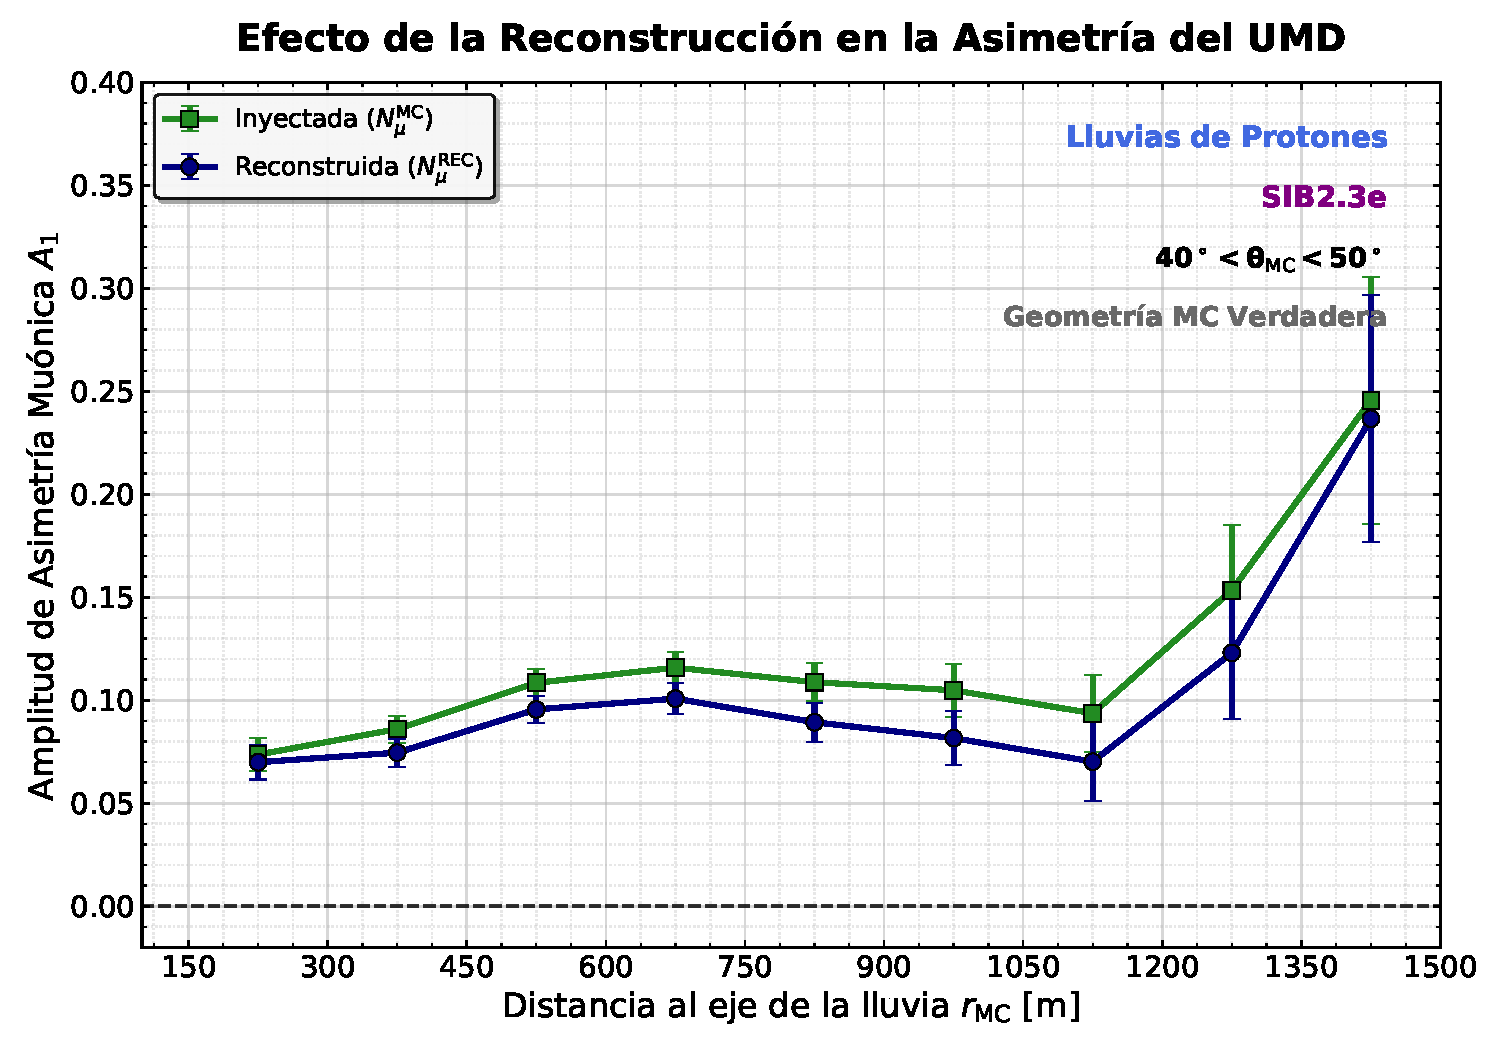
\includegraphics[width=1\textwidth]{capitulos/imagenes_capitulos/cap6/UMD_Asymmetry_MC_vs_REC.pdf}
	\caption{Comparación de la amplitud de asimetría $A_1$ obtenida a partir del número de muones inyectado ($N_\mu^{\mathrm{MC}}$) frente al número de muones reconstruido ($N_\mu^{\mathrm{REC}}$) para el rango cenital de referencia de $40^\circ \leq \theta < 50^\circ$. Ambas se realizan fijando las coordenadas a nivel Monte Carlo. Se observa que la respuesta instrumental del detector introduce una atenuación sistemática en la magnitud de la asimetría, preservando la evolución radial.}
	\label{fig:umd_rec_vs_mc_theta}
\end{figure}

\subsubsection{Competencia de observables: UMD frente al SD Total}
\label{subsubsec:umd_vs_sd_mc}

Con la fenomenología muónica del UMD caracterizada, el siguiente paso analítico consistió en contrastar este comportamiento frente a la señal total registrada por los tanques Cherenkov en superficie. Resulta importante realizar una distinción fundamental respecto a las variables físicas analizadas: mientras que el detector subterráneo proporciona un conteo directo del número de partículas muónicas incidentes reconstruidas, el SD registra la energía depositada en el volumen de agua, calibrada en unidades VEM, también a partir de la reconstrucción. Para garantizar la validez fenomenológica de este contraste, se mantuvo estrictamente la geometría Monte Carlo, asegurando que cualquier divergencia observada se deba puramente a la naturaleza de la señal detectada a nivel del suelo.

Si analizamos para el bin radial que incluye $\sim 450$~m se puede ver que, análogamente como sucedía para el Anillo Denso, la asimetría detectada por el SD es significativamente mayor a la del UMD. Ademas ambas asimetrías calculadas tienen magnitudes comparables a las encontradas en la sección del Anillo Denso. Esto permite ver que los analisis realizados en ambos marcos son comparables y consistentes.

Al extraer la amplitud de asimetría sobre la señal del SD, la curva resultante $A_1(r, \theta)$ expone un comportamiento espacial sistemáticamente distinto al del detector subterráneo. Como se evidencia en la Figura \ref{fig:umd_vs_sd_mc} para un rango cenital de referencia de $30^\circ \leq \theta < 40^\circ$, mientras que el UMD exhibe un crecimiento suave hacia una asimetría positiva a grandes distancias (aun en este rango cenital donde se ve un amecetamiento), el observable del SD presenta una pronunciada inversión fenomenológica. En el régimen donde el gradiente atmosférico debería garantizar una marcada asimetría positiva, la amplitud del SD alcanza un máximo local, comienza a suprimirse y finalmente se invierte, adoptando valores de asimetría fuertemente negativos en la periferia del centro de la lluvia. 

\begin{figure}[H]
	\centering
	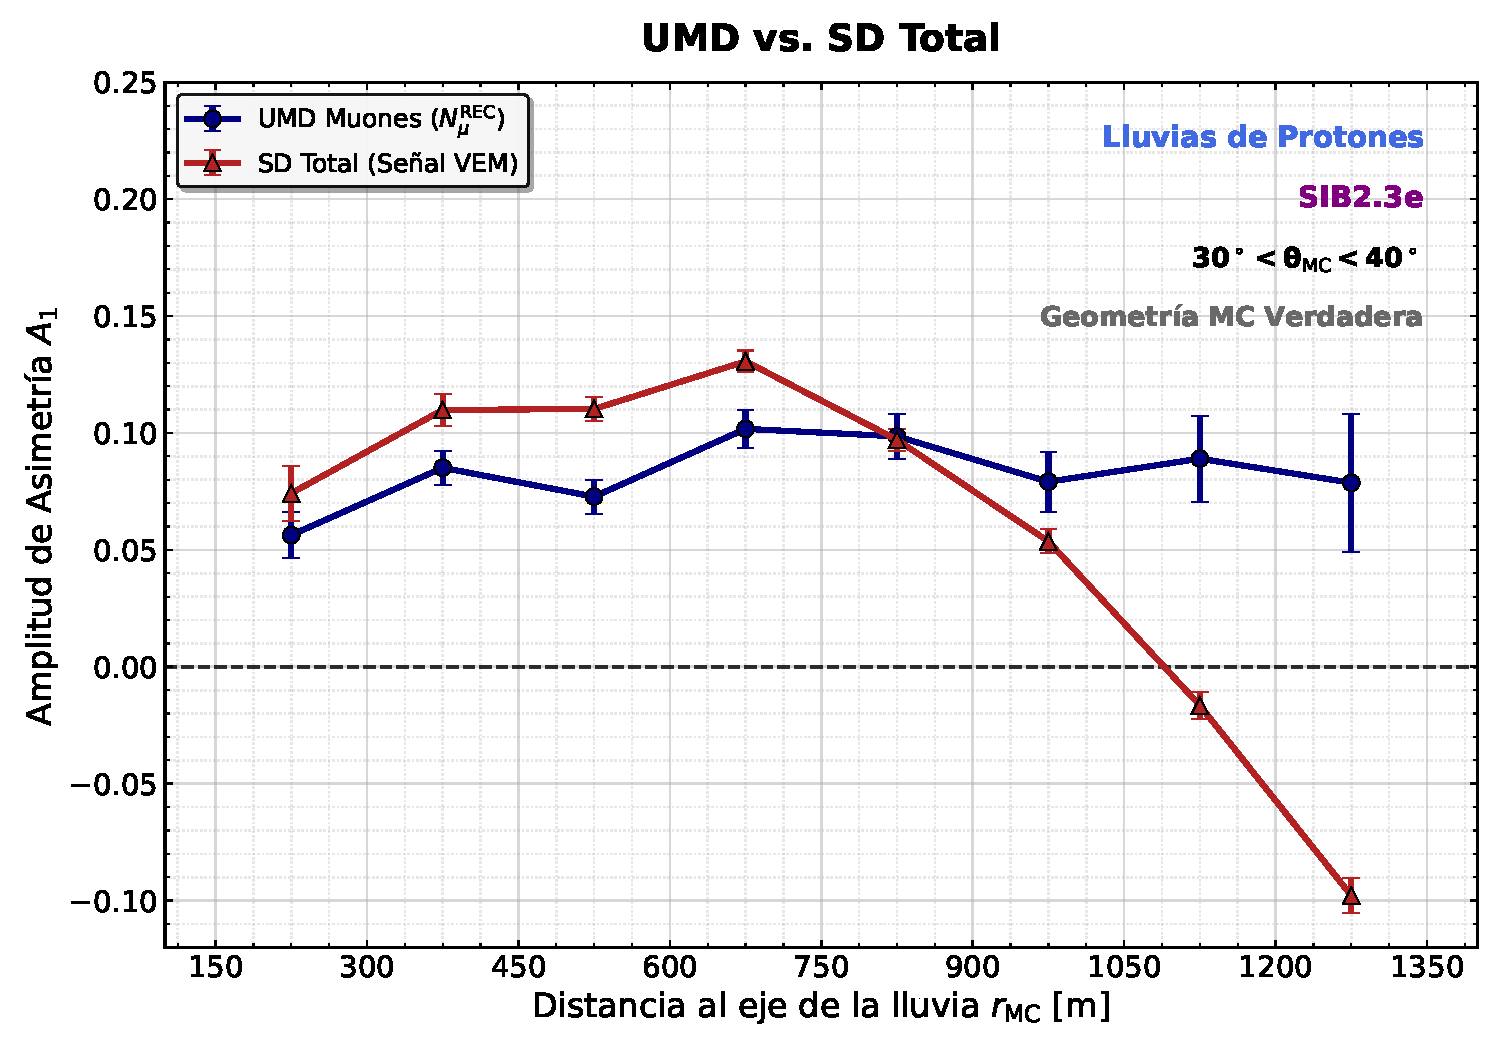
\includegraphics[width=1\textwidth]{capitulos/imagenes_capitulos/cap6/UMD_vs_SD_Total_Asymmetry.pdf}
	\caption{Comparación de la evolución radial de la amplitud de asimetría $A_1$ entre la componente muónica pura del UMD y la señal total registrada por los tanques del SD en superficie, evaluada para el rango cenital de referencia de $30^\circ \leq \theta < 40^\circ$. Ambas curvas fueron extraídas fijando la geometría real de Monte Carlo. Se evidencia el comportamiento divergente de los observables: mientras que el UMD presenta un incremento monótono condicionado por la atenuación, la señal del SD Total exhibe una severa disminucion de la asimetría que culmina en una inversión (asimetría negativa) en el \textit{far-core}.}
	\label{fig:umd_vs_sd_mc}
\end{figure}

Esta inversión geométrica no es un artefacto de reconstrucción, sino una propiedad física intrínseca de la cascada registrada a nivel del suelo, sugiriendo que el tanque Cherenkov integra poblaciones de partículas con asimetrías diametralmente opuestas.

\subsubsection{Desglose de señales: La inversión de la asimetría muónica}
\label{subsubsec:desglose_sd}

Para entender el origen físico del comportamiento anómalo del Detector de Superficie al compararse con el Subterráneo, se aprovechó la trazabilidad de las simulaciones para desglosar la señal VEM total en sus dos componentes formativas: la componente electromagnética (electrones y fotones) y la componente muónica medida a nivel del suelo. 

Cabe destacar que existe una diferencia sustancial en el tipo de señales que se están contrastando. La señal declarada como SD Total es la combinación energética de ambas componentes, pero es obtenida a través de la reconstrucción instrumental. Esta señal se calibra a partir de las trazas registradas en los fotomultiplicadores utilizando como referencia la medición del Muón Equivalente Vertical (VEM). En cambio, las componentes por separado que se analizan en esta sección representan la cantidad pura de partículas incidentes a nivel del suelo (nivel Monte Carlo). 

Al evaluar la asimetría de manera independiente para cada población, se descubre una competencia radial masiva, ilustrada en la Figura \ref{fig:desglose_sd_mc}. Por un lado, la componente electromagnética del SD exhibe una asimetría fuertemente positiva en todo el espectro radial. Dado que estas partículas se regeneran y absorben continuamente, su densidad está acoplada casi instantáneamente al perfil de desarrollo longitudinal de la cascada, convirtiéndolas en un trazador puro de la atenuación atmosférica. Se observa también un comportamiento singular: una estabilización (meseta) de la asimetría para todos los bines radiales por encima de los $\sim 600$~m. Si bien este fenómeno ocurre en diversas franjas cenitales, los estadísticos de bondad de ajuste en esta región profunda decrecen, lo que sugiere que la estabilización podría estar ligada a fluctuaciones estadísticas debido a la atenuación de la componente electromagnética a grandes distancias.

Por otro lado, la asimetría de los muones registrados por el SD exhibe un comportamiento transicional. Es aquí donde radica el mayor hallazgo analítico de esta comparación dado que el SD registra muones superficiales que, en los primeros bines radiales, se comportan de manera análoga al UMD (con una asimetría positiva creciente). Sin embargo, al acercarse a bines de mayor radio ($\sim 600$~m), la fenomenología cambia drásticamente y la magnitud de asimetría comienza a decrecer, invirtiendo su polaridad hacia valores fuertemente negativos en el \textit{far-core}. Este fenómeno condiciona por completo a la señal total del SD, evidenciando que, a grandes distancias del eje, la asimetría del tanque Cherenkov está dominada por la población muónica de superficie. Este fenómeno ya había sido descripto con anterioridad por la Colaboración.

El origen físico de esta inversión se explica de manera natural al recuperar la fenomenología desarrollada en la Sección \ref{subsubsec:divergencia}. Como se demostró, la asimetría azimutal resulta de la competencia directa entre la atenuación atmosférica y la dispersión geométrica de las partículas. El Detector de Superficie, al no poseer un umbral de energía relevante para los muones, se inunda abrumadoramente de la denominada Población B: muones de baja energía con un momento longitudinal muy bajo ($p_z \sim p_t$). 

Al estar la señal superficial dominada numéricamente por esta población altamente divergente, el tanque Cherenkov se vuelve extremadamente sensible a la excentricidad de la proyección del disco de la lluvia sobre el suelo inclinado. Como fue derivado analíticamente por Billoir, el ensanchamiento espurio de la región tardía está gobernado por el término asimétrico $\mathcal{A}_{geo}$ de la ecuación \ref{eq:efecto_geo}

Para la población de muones superficiales, el momento longitudinal $p_z$ es pequeño, provocando que el factor $\langle p_r / -p_z \rangle$ explote a grandes distancias radiales con valores negativos. En términos topológicos, la región tardía concentra una porción del haz divergente original intrínsecamente mucho más densa. Esta compresión geométrica genera una acumulación artificial de señal que supera holgadamente el vaciamiento físico producido por la atenuación atmosférica, forzando la asimetría global hacia el régimen negativo. En consecuencia, la inversión observada en el SD Total es el resultado determinista de convolucionar un frente electromagnético asimétrico positivo con este fondo muónico superficial dominado por el efecto geométrico.


\begin{figure}[H]
	\centering
	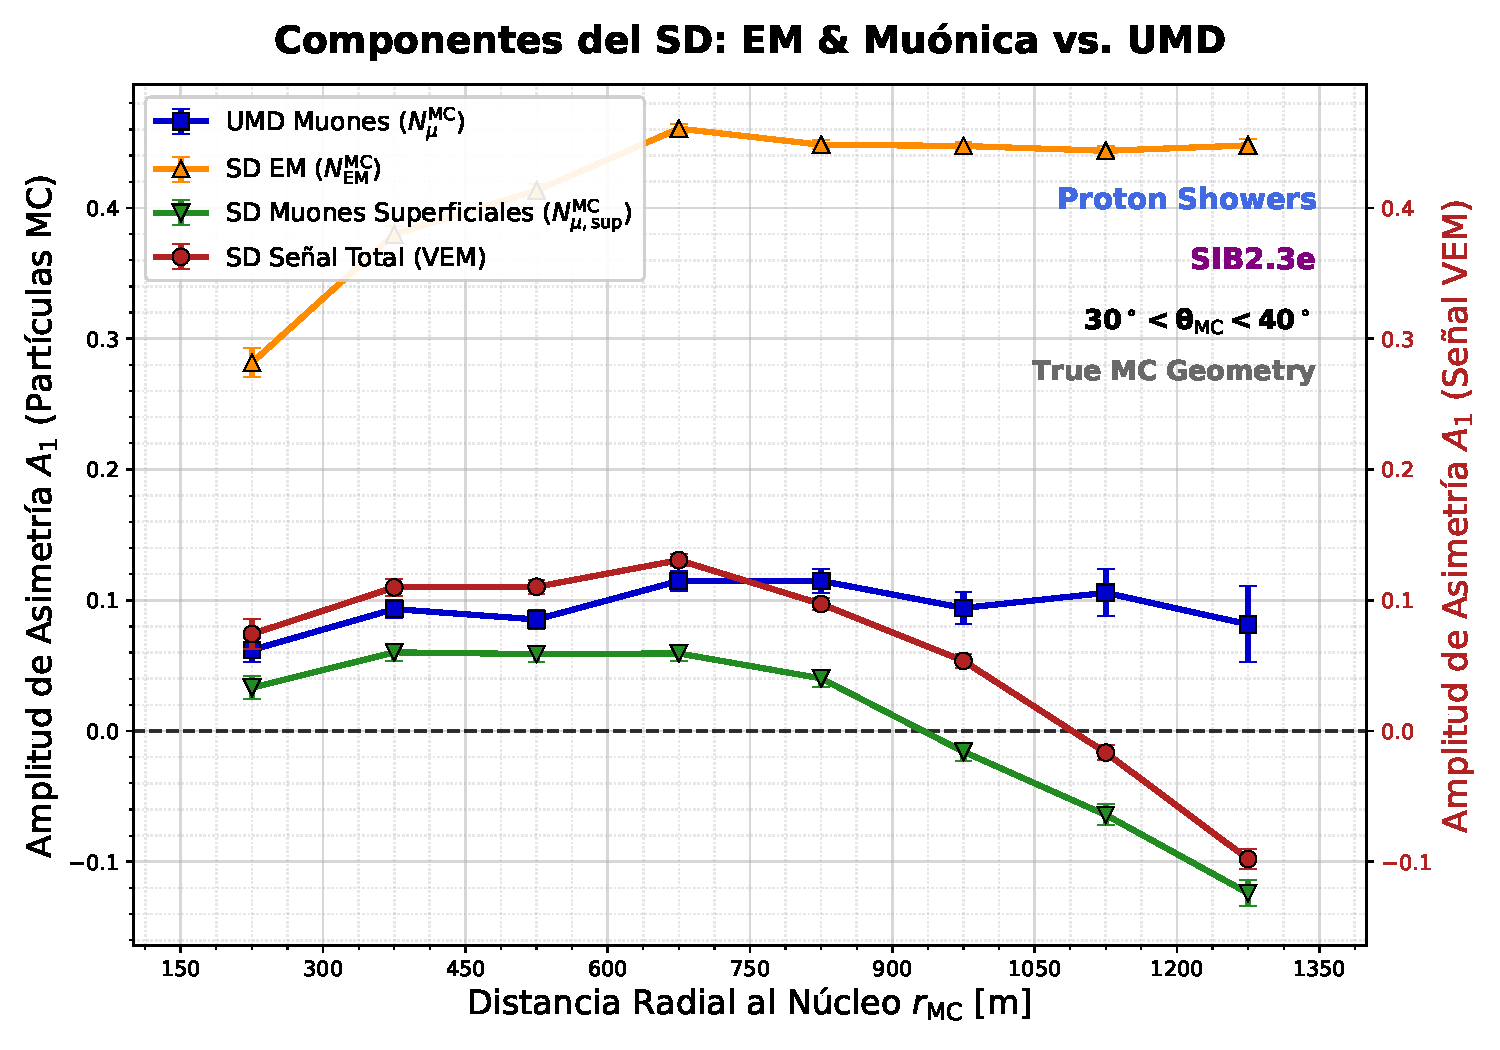
\includegraphics[width=1\textwidth]{capitulos/imagenes_capitulos/cap6/SD_Desglose_Componentes_vs_UMD.pdf}
	\caption{Desglose de la asimetría azimutal para las componentes inyectadas a nivel del suelo frente a la respuesta del detector subterráneo ($30^\circ \leq \theta < 40^\circ$). La asimetría electromagnética del SD (naranja) exhibe un comportamiento marcadamente positivo acoplado a la evolución longitudinal. En contraste, los muones superficiales del SD (verde) presentan una asimetría negativa a grandes distancias, producto del efecto de dispersión geométrica por proyección del disco \cite{Luce_ICRC2021}.}
	\label{fig:desglose_sd_mc}
\end{figure}

La comparación con el UMD valida empíricamente este modelo analítico y demuestra la superioridad instrumental del detector subterráneo. El blindaje pasivo de 2.3 m de tierra actúa como un filtro cinemático estricto, suprimiendo por completo a la población blanda divergente (Población B) y permitiendo únicamente el paso de muones altamente energéticos de la Población A ($E_\mu \gtrsim 1 \text{ GeV}$). De acuerdo a la relación cinemática, estos muones viajan en un haz altamente colimado donde el momento longitudinal es inmenso ($p_z \gg p_t$). 

Al imponer esta restricción física sobre el detector, el artefacto de proyección topográfica colapsa matemáticamente a cero ($\lim_{p_z \to \infty} \mathcal{A}_{geo} \to 0$). Al neutralizarse analíticamente el ensanchamiento radial excéntrico, el efecto asimétrico de compresión del disco pierde dominancia. De este modo, la atenuación longitudinal recupera el control del observable, lo que justifica la robusta y monótona asimetría positiva observada en la curva del detector subterráneo.

En conclusión, este desglose poblacional demuestra de manera irrefutable que la mera detección de la componente muónica en superficie no es suficiente para estudiar la direccionalidad global de la cascada. Se requiere de la atenuación de la tierra para suprimir los artefactos geométricos introducidos por la cinemática de baja energía, estableciéndose al UMD como un instrumento fenomenológicamente superior para aislar la asimetría longitudinal.

\subsubsection{Propuesta de Modelado del Filtro Cinemático}
\label{subsec:fast_mc}

Si bien el análisis de las simulaciones procesadas con el \textit{framework Offline} ha demostrado de manera contundente la degradación sistemática de la asimetría azimutal en el Detector de Superficie (SD) y su preservación en el Detector Subterráneo de Muones (UMD), la demostración del mecanismo propuesto en la sección anterior para explicar la competencia entre efectos y la diferencia fenomenológica entre detectores requiere un abordaje desde primeros principios. 

La limitación intrínseca de este estudio radica en que las simulaciones utilizadas entregan la huella final de la lluvia a nivel del suelo, careciendo de la granularidad necesaria para rastrear la cinemática de producción individual ($p_z$, $p_t$ y altura de decaimiento $z$) de cada partícula antes de su propagación. Para probar de manera aislada que la asimetría negativa es un artefacto geométrico exclusivo de la Población B y que el UMD lo anula por completo, se deja planteado como perspectiva a futuro, excediendo los alcances del presente trabajo, el desarrollo de un \textit{Toy Model} fenomenológico (un propagador \textit{Fast-Monte Carlo}).

La hoja de ruta propuesta para implementar este modelo en futuras investigaciones, el cual acoplaría la producción hadrónica con el transporte analítico de los muones, se estructuraría en las siguientes etapas:

\begin{enumerate}
	\item \textbf{Extracción de las distribuciones de producción:} Generar un lote de simulaciones dedicadas en CORSIKA con el único fin de extraer la función de distribución tridimensional en el punto de decaimiento del hadrón progenitor: $F(X, E_i, p_t)$. De esta forma, se obtiene el espectro de energía inicial y momento transversal real en función de la profundidad atmosférica $X$.
	
	\item \textbf{Propagación analítica y supervivencia:} A partir de $F(X, E_i, p_t)$, aplicar técnicas de remuestreo (\textit{Bootstrap} o Monte Carlo) para inyectar muones y propagarlos analíticamente hacia el suelo. Esta etapa utilizará el modelo de transporte cinemático de L. Cazón \textit{et al.} \cite{Cazon2012}, aplicando la isoterma atmosférica para calcular las pérdidas continuas de energía por ionización ($dE/dX$) y evaluar la probabilidad de supervivencia frente al decaimiento en vuelo.
	
	\item \textbf{Proyección geométrica e impacto:} Intersecar las trayectorias resultantes con el plano inclinado del arreglo de superficie. Este paso introducirá de forma natural la excentricidad geométrica, permitiendo evaluar cómo la divergencia radial de cada partícula afecta su fase azimutal de impacto.
	
	\item \textbf{El filtro instrumental:} Al obtener la energía final residual a nivel del suelo ($E_f$), se aplicarán funciones escalón para emular los diferentes umbrales instrumentales. Se evaluará la densidad total (emulando la respuesta muónica del SD) y se contrastará contra la distribución aplicando un umbral cinemático estricto de $E_f \gtrsim 1.0\text{ GeV}$ (emulando el blindaje pasivo del UMD).
\end{enumerate}

Una vez concretado en trabajos posteriores, este marco permitirá demostrar de forma completamente analítica cómo el espectro de baja energía, al poseer ángulos de divergencia masivos, dispara el término geométrico $\langle p_r / -p_z \rangle$ forzando la asimetría negativa ($A_1 < 0$) en el \textit{far-core}. Simultáneamente, probará desde las ecuaciones fundamentales de transporte que la barrera de atenuación del UMD filtra las trayectorias de bajo momento longitudinal, anulando la distorsión proyectiva de manera determinista y revelando únicamente la asimetría positiva intrínseca al desarrollo longitudinal de la lluvia.

\subsection{Arreglo \textit{Infill} usando la geometría reconstruida}
\label{subsec:infill_rec}

Habiendo caracterizado la fenomenología pura de la cascada utilizando el escenario ideal (núcleo y ángulos Monte Carlo), el análisis se traslada en el contexto de simulaciones al entorno experimental más realista posible. En esta sección, el cálculo de las coordenadas y fases azimutales en el plano de la lluvia se realiza utilizando la posición del centro de impacto y los ángulos de arribo reportados por el algoritmo de reconstrucción del Observatorio (geometría \textit{REC}).

Al igual que en el estudio con geometría ideal, la transición de utilizar la cantidad de muones inyectados ($N_\mu^{\mathrm{MC}}$) a la de muones reconstruidos por la electrónica del UMD ($N_\mu^{\mathrm{REC}}$) conserva la forma de la evolución de la asimetría, solo afectando débilmente su magnitud debido a los sesgos direccionales del algoritmo. Sin embargo, al introducir la incertidumbre espacial de la \textbf{geometría reconstruida}, el panorama fenomenológico cambia drásticamente para todos los detectores: la modulación azimutal se ve severamente comprometida, perdiéndose la capacidad de detectar asimetría en diversas regiones radiales.

El análisis sistemático de los ajustes armónicos sobre los datos reconstruidos permite mapear de manera transparente los límites resolutivos y estadísticos del arreglo \textit{Infill} al menos en el marco de simulaciones:

\begin{itemize}
	\item \textbf{Régimen cuasi-vertical ($0^\circ \le \theta < 20^\circ$):} La asimetría es físicamente marginal y la reconstrucción apenas logra identificar modulaciones débiles en un rango acotado ($450 \le r \le 1050\text{ m}$). Fuera de esta ventana, las fluctuaciones dominan sobre el gradiente direccional.
	
	\item \textbf{Régimen de transición ($20^\circ \le \theta < 40^\circ$):} Se establece una clara ventana de máxima fidelidad fenomenológica entre los $650\text{ m}$ y los $1200\text{ m}$. Los ajustes armónicos convergen con valores de $\chi^2/\mathrm{ndf}$ estables y barras de error acotadas pero la magnitud de la asimetria es baja y y no sigue el comportamiento esperado de aumentar a medida que el bin radial aumenta. Para distancias superiores ($r > 1200\text{ m}$), la densidad muónica decae drásticamente.
	
	\item \textbf{Régimen de alta inclinación ($50^\circ \le \theta < 65^\circ$):} Debido a la inmensa proyección del disco muónico sobre el suelo para lluvias rasantes, la estadística de conteo se mantiene elevada a grandes distancias. Esto permite que el ajuste armónico sobreviva con notable estabilidad y magnitud desde los $600\text{ m}$ hasta la periferia más lejana del arreglo ($1500\text{ m}$), consolidando a este rango como el escenario óptimo para el estudio de asimetrías de atenuación en el \textit{far-core}.
\end{itemize}

Este fenómeno de degradación responde a una difusión o \textit{smearing} angular. La incertidumbre espacial intrínseca en la determinación del núcleo del arreglo \textit{Infill} ($\sigma_{core} \approx 20 - 40$~m) propaga un error continuo en el cálculo del azimut asignado a cada estación ($\Delta \phi$). Estadísticamente, esto implica que estaciones que físicamente pertenecen a la región temprana pura ($\phi \approx 0^\circ$) son erróneamente catalogadas con fases laterales, y viceversa. Esta mezcla espuria de poblaciones modera los máximos y mínimos de la distribución de densidad, actuando como un filtro pasa-bajos espacial que "plancha" la modulación cosenoidal. El efecto es especialmente destructivo cerca del núcleo ($r \lesssim 400$~m), donde un leve corrimiento del centro de impacto invierte por completo el vector de posición, justificando la necesidad estricta del corte fiducial aplicado.



\subsubsection{Resiliencia de la componente electromagnética en la reconstrucción}

Al repetir el análisis de competencia entre el UMD y el SD, pero ahora sujetos a la degradación geométrica de la reconstrucción, emerge una conclusión inesperada al desglosar la señal del tanque Cherenkov. 

A pesar de que el \textit{smearing} angular destruye gran parte de la modulación en la componente muónica del UMD y del SD, el ajuste armónico sobre la componente electromagnética (SD EM) revela que esta preserva una asimetría fuertemente positiva y altamente significativa a lo largo de todos los bines radiales evaluados. Aún bajo los efectos de la incertidumbre topográfica, la señal EM se ajusta con barras de error estadístico notablemente pequeñas.

Esta excepcional resiliencia no implica que los fotones y electrones sean inmunes al error de reconstrucción, sino que es una consecuencia directa de su abrumadora abundancia estadística. La componente electromagnética es órdenes de magnitud más numerosa que la muónica y experimenta un gradiente de atenuación longitudinal sumamente pronunciado. La asimetría física generada por este vaciamiento atmosférico es tan profunda y estadísticamente rica que logra sobreponerse a la "borrosidad" espacial introducida por el desplazamiento del núcleo.

\subsubsection{La supervivencia de la asimetría geométrica muónica}

Por el contrario, la inversión de la asimetría del observable total del SD hacia valores negativos en el \textit{far-core} se sigue manifestando con total contundencia en los datos reconstruidos. Esta inversión encuentra su justificación en la naturaleza de la parte muónica del SD.

Como se desarrolló en la sección analítica, la asimetría negativa es impulsada por la población de muones blandos que inunda los detectores de superficie. Debido a su enorme divergencia ($p_t \sim p_z$), el término de asimetría geométrica de Billoir ($\mathcal{A}_{geo} \propto \langle p_r / -p_z \rangle$) explota a grandes distancias radiales. La compresión geométrica sufrida por esta porción del haz en la región tardía es tan masiva que el exceso de partículas sobrevive sin problemas al difuminado de la reconstrucción angular. De esta forma, un frente electromagnético positivo (resistente por su altísima estadística) compite contra un fondo de muones blandos fuertemente negativos (resistentes por la escala masiva de su divergencia). El resultado de esta convolución es la caída y posterior inversión a valores negativos del SD Total, confirmando que este artefacto no es una falla de Monte Carlo, sino un obstáculo experimental empírico.

\subsection{Comparación de performance: UMD Monte Carlo vs. UMD Reconstruido}
\label{subsec:comparacion_performance_umd}

Habiendo justificado el comportamiento del SD, el foco recae finalmente sobre la performance del Detector Subterráneo de Muones frente a las incertezas de la reconstrucción. Al comparar directamente los ajustes obtenidos para el UMD utilizando la geometría Monte Carlo contra aquellos obtenidos con la geometría Reconstruida, se consolida una métrica del poder resolutivo del instrumento.

% ACÁ PODÉS INSERTAR LA COMPARACIÓN DE PERFORMANCE DEL UMD. 
% Sugerencia de cómo engancharlo:
La comparativa evidencia que, si bien el UMD logra filtrar cinemáticamente a la población blanda y aislar la asimetría positiva en el mundo ideal, la introducción de los errores de reconstrucción del arreglo de superficie (Core REC) impone una cota experimental a la amplitud observable. La difusión angular "achata" las curvas de $A_1$, indicando que las asimetrías medidas experimentalmente representarán sistemáticamente un límite inferior (\textit{lower bound}) de la verdadera polaridad de la cascada. Maximizar la precisión algorítmica en la ubicación del núcleo resulta, por lo tanto, tan determinante para medir la atenuación como lo es el propio blindaje del detector.


---


DESPUES PASAMOS A HABLAR DE LO MISMO PERO USANDO CORE Y ANGULOS REC

ACA SE PUEDE MEZCLAR UN POCO LO DE DIVIDIR EN SUBSUB CAPTIRULOS PERO, DECIR Q NUEVAMENTE LA RECONSTRUCCION DE LA CANTIDAD DE MUONES NO AFECTA LA FENOMENOLOGIA DE COMO CAMBIA LA ASIMETRIA (TAL VEZ SOLO UN POCO EN MAGINTUD IGUAL Q ANTES), PERO QUE PARA AMBOS DEJAMOS DE VER ASIMETRIA (HABLAR BIEN DE CUANDO)

DECIR QUE SE REPITE LO MISMO CUANDO SE COMAPRA UMD CON SD PERO QUE AHORA SE LLEGO A UNA CONCLUSION QUE SORPENDIO EN EL DESLGOSE DEL SD. QUE AUN EN LA RE4CONSTRUCCION SE VE SIEMPRE SUPER SIGNIFICATIVO QUE PARA EL SD EM SE VE LA ASIMETRIA RE FUERTTE Y CON MUY POCO ERROR PARA TODOS LOS BINES RADIALES



Y RECIEN DESPUES DE TODO ESTO PASARIA A HABLAR DE LA COMPARACION DE LA PREFORMANCE DEL REC VS MC EN CORE Y ANGULOS, PPALMENTE HABLANDO DEL UMD. ACA NO ME QUEDA CLARO COMO HARIA ESTA COMPARACION TODAVIA

Y HABRIA QUE VER SI SE PUEDE METER ALGO DE LA JUSTIFICAICON DE LA INVERSION DE ASIMETRIA EN EL SD CAUSADDA POR LA INVERSION DE ASIMETRIA DE LA PARTE MUONICA DEL SD QUE SE VE EN TANTO REC COMO MC. UNA EXPLCAICION, UN TOY MODEL O ALGO ASI



 IDEAS:
 
 VER SI PUEDO AGREGAR A A1(R, THETA) UNA DEPENDENCIA CON PRIMARIO Y ENERGIA. PARA ESTO TENGO QUE VER PRIMERO:
 
 1. SI PIERDO MUCHA ESTADTSITCA HACIENDO UN BINEADO EN ENERGIA EN 5 BINES COMO EN LA SECCION DEL UMD
 
 2. PROBAR QUE PASA SI HAGO EL MSMO ESTUDIO CON LOS DATOS DE HIERRO
 
 TODO ESTO LO HARIA EN UNA SESCCION APARTE Y LAS SUBSECCION SERIAN VER QUE PASA CON LA PARTE USANDO COSAS MC Y CON LA REC
 
 
 
 PODRIA VER QUE ONDA TAMBIEN LO DEL ANGULO DE INCIDENCIA O MERAMENTE DECLARARLO, PORQUE PARA MOSTRAR UN PLOT CHATO NO VALE NADA, Y ADEMAS TENGO POCA SENSIBILIDAD ENTONCES PUEDE SER QU ED EMEDIO RARO
 

\newpage

\clearpage
\printbibliography
\end{document}
